% !TeX root = ../tfg.tex
% !TeX encoding = utf8

\chapter{Resultados experimentales}

\section{Rendimiento y selección de modelos}

A continuación se presentan los resultados de las métricas respecto a los conjuntos de validación obtenidas tras el entrenamiento de las redes. El objetivo de esta sección será seleccionar los modelos que emplearemos para comparar la evolución de la homología persistente entre ellos.

\subsection{Selección de hiperparámetros}
\label{subsec:hiperparam}

La \autoref{fig:loss-optim-m} muestra la evolución de la función de pérdida promedio respecto al optimizador a lo largo del entrenamiento. En ella, podemos observar que los modelos entrenados con SGD para los distintos tamaños de lote y arquitecturas han mostrado unas tasas de pérdida más bajas y mayor regularidad en el conjunto de validación. En general, la gráfica muestra un desarrollo correcto del proceso de entrenamiento.

\begin{figure}[H]
		\centering
		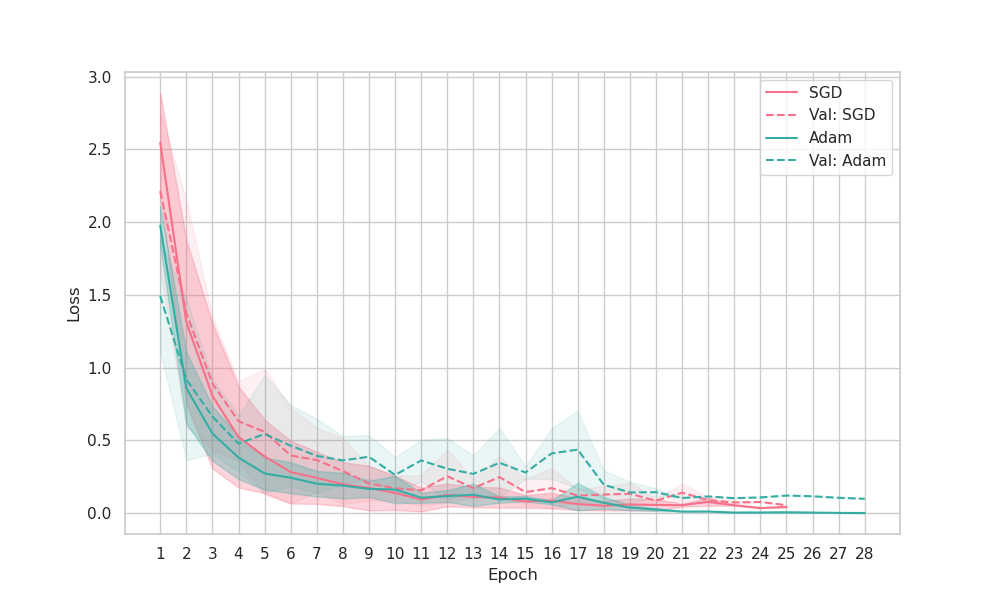
\includegraphics[width=0.8\textwidth]{img/loss-optimizer-marca.png}
		\caption{Función de pérdida promedio en entrenamiento y validación de los distintos modelos entrenados en función del optimizador empleado: SGD y Adam. Se muestra de forma sombreada la desviación típica de la función de pérdida.}
		\label{fig:loss-optim-m}
\end{figure}

Por otro lado, la \autoref{fig:loss-batch-m} muestra como existe una mayor variabilidad en el proceso de entrenamiento entre los modelos con un mismo tamaño de lote. Entre ellos, el que parece presentar una mayor estabilidad para las distintas arquitecturas es con un tamaño de lote 64, pues muestra una menor desviación típica y valores bajos en la función de pérdida.

\begin{figure}[H]
	\centering
	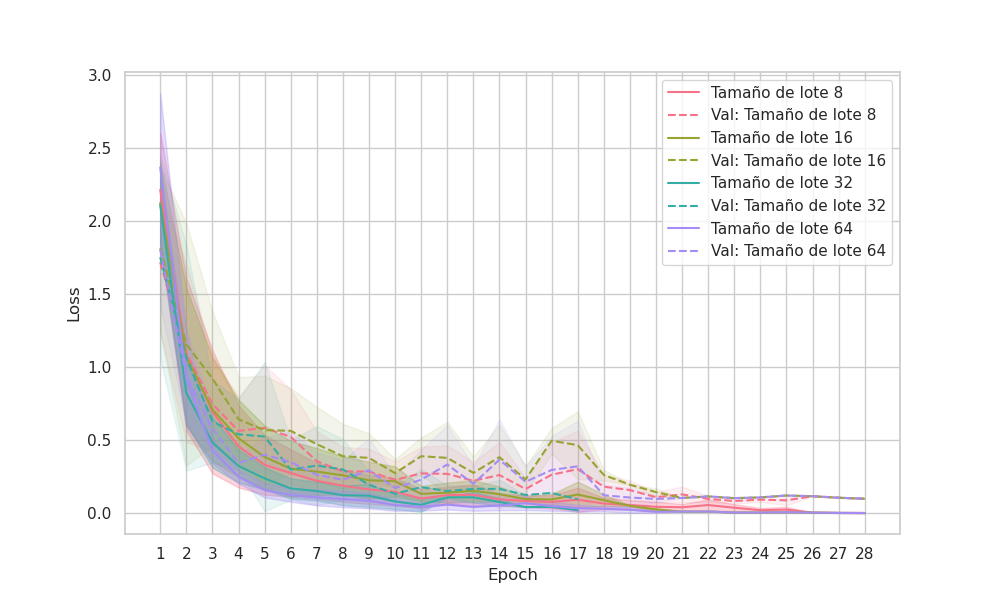
\includegraphics[width=0.8\textwidth]{img/loss-batch-marca.png}
	\caption{Función de pérdida promedio en entrenamiento y validación de los distintos modelos entrenados en función delos tamaños de lote empleados: 8, 16 ,32 y 64. Se muestra de forma sombreada la desviación típica de la función de pérdida.}
	\label{fig:loss-batch-m}
\end{figure}

Finalmente, las figuras \ref{fig:loss-optim-mm} y \ref{fig:loss-batch-mm}, muestran un comportamiento similar a las recién vistas, indicando un correcto desarrollo de la fase de entrenamiento. A diferencia de las anteriores, si bien SGD ha vuelto a mostrar una mejor evolución de la curva de pérdida, es esta vez el tamaño de lote 32 el que ha mostrado unas tasas de pérdida promedio más baja. Otra observación interesante es la disminución en la pendiente de la curva, reflejando una mayor dificultad en el aprendizaje en la especificidad Marca-Modelo.

\begin{figure}[H]
	\centering
	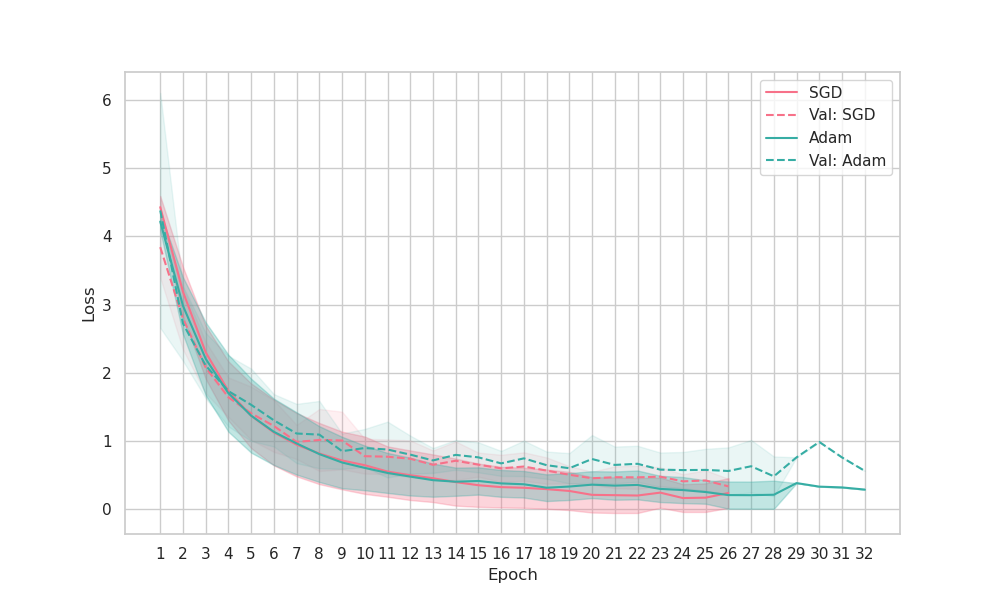
\includegraphics[width=0.8\textwidth]{img/loss-optimizer-marca-modelo.png}
	\caption{Función de pérdida promedio en entrenamiento y validación de los distintos modelos entrenados en función del optimizador empleado: SGD y Adam. Se muestra de forma sombreada la desviación típica de la función de pérdida.}
	\label{fig:loss-optim-mm}
\end{figure}

\begin{figure}[H]
	\centering
	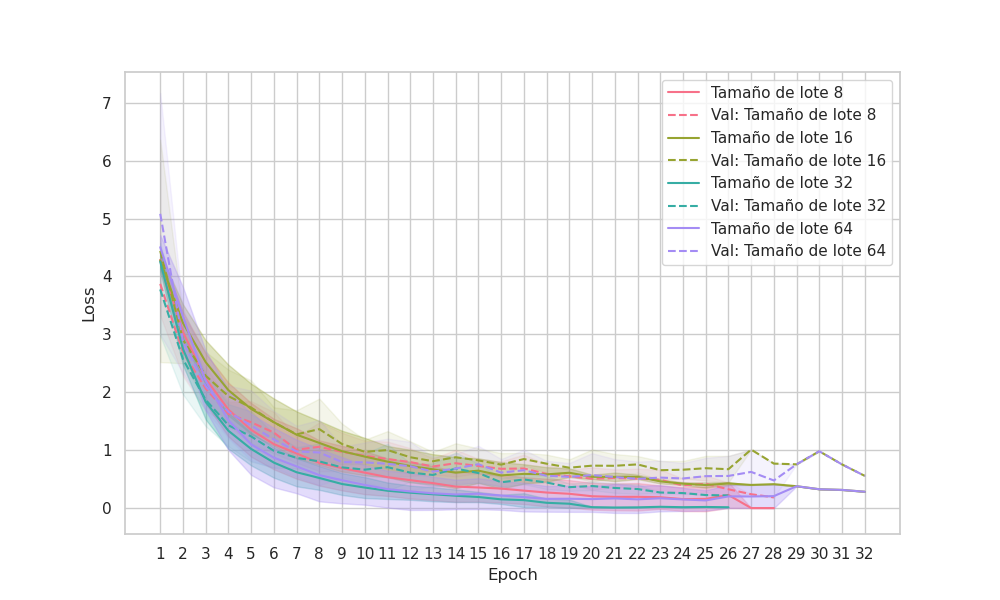
\includegraphics[width=0.8\textwidth]{img/loss-batch-marca-modelo.png}
	\caption{Función de pérdida promedio en entrenamiento y validación de los distintos modelos entrenados en función de los tamaños de lote empleados: 8, 16 ,32 y 64. Se muestra de forma sombreada la desviación típica de la función de pérdida.}
	\label{fig:loss-batch-mm}
\end{figure}

Las Tablas \ref{tab:sgd_metrics-marca} y \ref{tab:adam_metrics-marca} muestran las métricas obtenidas durante el proceso de entrenamiento tanto para SGD como Adam respectivamente para la especificidad de Marca. Todas ellas han alcanzado el criterio de parada en menos de 2 horas y de 50 épocas. En general, podemos observar que ambos optimizadores logran una puntuación superior al $95\%$ en la gran mayoría de las métricas. Es interesante observar cómo pese al desbalance de los datos, el F1-Score sigue mostrando resultados excelentes. Entre todos los modelos vemos que los mejores resultados los ha obtenido EfficientNet-B0 con el optimizador SGD y un tamaño de lote 8 y 64. Sin embargo, finalmente se ha optado por escoger el mismo modelo con un tamaño de lote 64, pues su resultados son muy similares y su F1-Score es ligeramente mayor.

\begin{table}[H]
	\begin{adjustbox}{width=1\textwidth}
		\begin{tabular}{|c|c|c|c|c|c|}
			\hline
			\textbf{Modelo} & \textbf{Tamaño de Lote} & \textbf{Exactitud} & \textbf{Precisión} & \textbf{Sensibilidad} & \textbf{F1-Score} \\
			\hline
			 & 8 & 0.9536 & 0.9416 & 0.9474 & 0.9443 \\ \cline{2-6}
			ResNet-18 & 16 & 0.9102 & 0.8834 & 0.8953 & 0.8891 \\ \cline{2-6}
			& 32 & 0.9721 & 0.9785 & 0.9753 & 0.9769 \\ \cline{2-6}
			& 64 & 0.9814 & 0.9758 & 0.9775 & 0.9767 \\
			\hline
			 & 8 & 0.9814 & 0.9850 & 0.9828 & 0.9838 \\ \cline{2-6}
			DenseNet-121 & 16 & 0.9752 & 0.9755 & 0.9783 & 0.9768 \\ \cline{2-6}
			 & 32 & 0.9845 & 0.9931  & 0.9863 & 0.9897 \\ \cline{2-6}
			 & 64 & 0.9814 & 0.9738 & 0.9753 & 0.9746 \\
			\hline
			 & 8 & \textbf{0.9907} & 0.9907 & \textbf{0.9917} & 0.9911 \\ \cline{2-6}
			EfficientNet-B0 & 16 & 0.9474 & 0.9512 & 0.9515 & 0.9512 \\ \cline{2-6}
			 & 32 & 0.9690 & 0.9798 & 0.9689 & 0.9743 \\ \cline{2-6}
			 & 64 & 0.9859 & \textbf{0.9925} & 0.9907 & \textbf{0.9916} \\
			\hline
		\end{tabular}
	\end{adjustbox}
	\caption{Métricas de validación para los modelos optimizados con SGD en la especificidad Marca.}
	\label{tab:sgd_metrics-marca}
\end{table}



\begin{table}[H]
	\begin{adjustbox}{width=1\textwidth}
		\begin{tabular}{|c|c|c|c|c|c|}
			\hline
			\textbf{Modelo} & \textbf{Tamaño de Lote} & \textbf{Exactitud} & \textbf{Precisión} & \textbf{Sensibilidad} & \textbf{F1-Score} \\
			\hline
			 & 8 & 0.9536 & 0.9496 & 0.9508 & 0.9501 \\ \cline{2-6}
			ResNet-18 & 16 & 0.9536 & 0.9486 & 0.9467 & 0.9475 \\ \cline{2-6}
			& 32 & 0.9381 & 0.9319 & 0.9235 & 0.9275 \\ \cline{2-6}
			& 64 & 0.9721 & 0.9713 & 0.9633 & 0.9672 \\
			\hline
			 & 8 & 0.9350 & 0.9428 & 0.9363 & 0.9393 \\ \cline{2-6}
			DenseNet-121 & 16 & 0.9536 & 0.9465 & 0.9463 & 0.9462 \\ \cline{2-6}
			 & 32 & 0.9659 & 0.9750 & 0.9694 & 0.9721 \\ \cline{2-6}
			 & 64 & \textbf{0.9876} & \textbf{0.9916} & \textbf{0.9869} & \textbf{0.9892} \\
			\hline
			 & 8 & 0.9598 & 0.9588 & 0.9576 & 0.9580 \\ \cline{2-6}
			EfficientNet-B0 & 16 & 0.9752 & 0.9768 & 0.9757 & 0.9762 \\ \cline{2-6}
			 & 32 & 0.9783 & 0.9720 & 0.9698 & 0.9709 \\ \cline{2-6}
			 & 64 & 0.9567 & 0.9330 & 0.9332 & 0.9331 \\
			\hline
		\end{tabular}
	\end{adjustbox}
	\caption{Métricas de validación para los modelos optimizados con Adam en la especificidad Marca.}
	\label{tab:adam_metrics-marca}
\end{table}

Por otro lado, los modelos entrenados sobre el conjunto de datos Marca-Modelo han mostrado mayores dificultades durante el proceso de aprendizaje, tal y como muestran los resultados de las Tablas \ref{tab:sgd_metrics_mm} y \ref{tab:adam_metrics_mm}. Pese a ello, la configuración que ha mostrado mejores resultados en las métricas evaluadas ha sido DenseNet-121 con SGD y un tamaño de lote 32. Esta configuración ha mostrado ser la mejor tanto en exactitud como en F1-Score, además de tener resultados competentes en el resto de métricas. Por ello, emplearemos dicho modelo en las siguientes etapas.

\begin{table}[H]
	\centering
	\begin{adjustbox}{width=\textwidth}
		\begin{tabular}{|c|c|c|c|c|c|}
			\hline
			\textbf{Modelo} & \textbf{Tamaño de Lote} & \textbf{Exactitud} & \textbf{Precisión} & \textbf{Sensibilidad} & \textbf{F1-Score} \\
			\hline
			& 8 & 0.8000 & 0.7934 & 0.7968 & 0.7949 \\ \cline{2-6}
			ResNet-18 & 16 & 0.8037 & 0.7866 & 0.7969 & 0.7916 \\ \cline{2-6}
			& 32 & 0.9000 & 0.8743 & 0.8912 & 0.8826 \\ \cline{2-6}
			& 64 & 0.8741 & 0.8510 & 0.8540 & 0.8524 \\
			\hline
			& 8 & 0.8667 & 0.8569 & 0.8624 & 0.8595 \\ \cline{2-6}
			DenseNet-121 & 16 & 0.8741 & 0.8739 & 0.8732 & 0.8734 \\ \cline{2-6}
			& 32 & \textbf{0.9407} & \textbf{0.9176} & \textbf{0.9314} & \textbf{0.9243} \\ \cline{2-6}
			& 64 & 0.9111 & 0.8985 & 0.9009 & 0.8997 \\
			\hline
			& 8 & 0.9111 & 0.9122 & 0.9116 & 0.9118 \\ \cline{2-6}
			EfficientNet-B0 & 16 & 0.8000 & 0.8020 & 0.8066 & 0.8040 \\ \cline{2-6}
			& 32 & 0.9148 & 0.9213 & 0.9181 & 0.9197 \\ \cline{2-6}
			& 64 & 0.9000 & 0.8941 & 0.8920 & 0.8929 \\
			\hline
		\end{tabular}
	\end{adjustbox}
	\caption{Métricas de validación para los modelos optimizados con SGD en la especificidad Marca-Modelo.}
	\label{tab:sgd_metrics_mm}
\end{table}

\begin{table}[H]
	\centering
	\begin{adjustbox}{width=\textwidth}
		\begin{tabular}{|c|c|c|c|c|c|}
			\hline
			\textbf{Modelo} & \textbf{Tamaño de Lote} & \textbf{Exactitud} & \textbf{Precisión} & \textbf{Sensibilidad} & \textbf{F1-Score} \\
			\hline
			 & 8 & 0.8556 & 0.8526 & 0.8536 & 0.8529 \\ \cline{2-6}
			ResNet-18 & 16 & 0.8556 & 0.8471 & 0.8543 & 0.8506 \\ \cline{2-6}
			& 32 & 0.7741 & 0.7367 & 0.7561 & 0.7461 \\ \cline{2-6}
			& 64 & 0.8556 & 0.8493 & 0.8438 & 0.8464 \\
			\hline
			 & 8 & 0.8741 & 0.8672 & 0.8725 & 0.8696 \\ \cline{2-6}
			DenseNet-121 & 16 & 0.8667 & 0.8685 & 0.8687 & 0.8685 \\ \cline{2-6}
			 & 32 & 0.9037 & 0.8943 & 0.9018 & 0.8979 \\ \cline{2-6}
			 & 64 & \textbf{0.9201} & \textbf{0.9263} & 0.9103 & \textbf{0.9182} \\
			\hline
			 & 8 & 0.8481 & 0.8384 & 0.8460 & 0.8420 \\ \cline{2-6}
			EfficientNet-B0 & 16 & 0.8926 & 0.8946 & 0.8924 & 0.8935 \\ \cline{2-6}
			 & 32 & 0.9148 & 0.9044 & \textbf{0.9143} & 0.9093 \\ \cline{2-6}
			 & 64 & 0.8111 & 0.7869 & 0.7906 & 0.7887 \\
			\hline
		\end{tabular}
	\end{adjustbox}
	\caption{Métricas de validación para los modelos optimizados con Adam en la especificidad Marca-Modelo.}
	\label{tab:adam_metrics_mm}
\end{table}

\subsection{Selección de transformaciones de datos}

Tras la anterior etapa se ha procedido a realizar un aumento de datos sobre los dos conjuntos seleccionados: EfficientNet-B0 con SGD y un tamaño de lote 64 para la especificidad Marca, y DenseNet-121 con SGD y tamaño de lote 32 para la especificidad Marca-Modelo. Las Tablas \ref{tab:transformation_metrics-m} y \ref{tab:transformation_metrics-mm} muestran los resultados obtenidos para cada una de las transformaciones descritas en la \autoref{sec:data-aug}.

Si bien el modelo entrenado para el conjunto de datos Marca con las transformaciones no ha mejorado significativamente, vemos que las transformaciones sobre el modelo entrenado para Marca-Modelo han logrado unas mejoras notablemente. El objetivo del aumento de datos en las CNNs es mejorar la capacidad de generalización de los modelos. Sin embargo, el primer modelo ya gozaba de muy buenas métricas por lo que un empeoramiento general al realizar aumento de datos podría significar un sobreajuste del modelo. Por tanto, entrenaremos el modelo de nuevo con las transformaciones que mejor hayan funcionado para estudiar cómo afectan a la topología.

\begin{table}[H]
	\centering
	\begin{adjustbox}{width=0.8\textwidth}
	\begin{tabular}{|c|c|c|c|c|c|}
		\hline
		\textbf{Transformación} & \textbf{Exactitud} & \textbf{Precisión} & \textbf{Sensibilidad} & \textbf{F1-Score} \\
		\hline
		Fluctuación & \textbf{0.9814} & \textbf{0.9869} & \textbf{0.9844} & \textbf{0.9856} \\
		\hline
		Desenfoque & 0.9567 & 0.9360 & 0.9388 & 0.9373 \\
		\hline
		Simetría & 0.9721 & 0.9634 & 0.9585 & 0.9609 \\
		\hline
		Recorte & 0.9783 & 0.9765 & 0.9709 & 0.9737 \\
		\hline
		Rotación & 0.9783 & 0.9706 & 0.9657 & 0.9682 \\
		\hline
	\end{tabular}
\end{adjustbox}
\caption{Métricas de validación para EfficientNet-B0 con transformaciones de datos en la especificidad Marca.}
\label{tab:transformation_metrics-m}
\end{table}

\begin{table}[H]
	\centering
	\begin{adjustbox}{width=0.8\textwidth}
	\begin{tabular}{|c|c|c|c|c|c|}
		\hline
		\textbf{Transformación} & \textbf{Exactitud} & \textbf{Precisión} & \textbf{Sensibilidad} & \textbf{F1-Score} \\
		\hline
		Fluctuación & 0.9783 & 0.9728 & 0.9745 & 0.9736 \\
		\hline
		Desenfoque & 0.9783 & 0.9790 & 0.9750 & 0.9769 \\
		\hline
		Simetría & 0.9814 & 0.9804 & 0.9775 & 0.9789 \\
		\hline
		Recorte & 0.9845 & 0.9863 & 0.9817 & 0.9840 \\
		\hline
		Rotación & \textbf{0.9876} & \textbf{0.9914} & \textbf{0.9874} & \textbf{0.9894} \\
		\hline
	\end{tabular}
\end{adjustbox}
\caption{Métricas de validación para DenseNet-121 con transformaciones de datos en la especificidad Marca-Modelo.}
\label{tab:transformation_metrics-mm}
\end{table}

Finalmente, la \autoref{tab:model_comparison_val} muestra los resultados de los modelos reentrenados con las transformaciones escogidas: EfficientNet-B0 con fluctuaciones en el color, recortes aleatorios y rotaciones aleatorias en Marca; y DenseNet-121 con todas las transformaciones propuestas en Marca-Modelo.

\begin{table}[H]
	\centering
	\begin{adjustbox}{width=0.85\textwidth}
		\begin{tabular}{|c|c|c|c|c|}
			\hline
			\textbf{Modelo} & \textbf{Exactitud} & \textbf{Precisión} & \textbf{Sensibilidad} & \textbf{F1-Score} \\
			\hline
			EfficientNet-B0 Trans (Marca) & 0.9505 & 0.9627 & 0.9501 & 0.9562 \\
			\hline
			\hline
			DenseNet-121 Trans (Marca-Modelo) & 0.7962 & 0.7660 & 0.7769 & 0.7712 \\
			\hline
		\end{tabular}
	\end{adjustbox}
	\caption{Rendimiento final de los modelos con aumento de datos en el conjunto de validación para EfficientNet-B0 en la especificidad Marca y para DenseNet-121 en la especificidad Marca-Modelo.
	}
	\label{tab:model_comparison_val}
\end{table}

Una vez obtenidos los modelos, podemos observar en la \autoref{tab:model_comparison_test_aug} las métricas obtenidas en cada modelo en el conjunto de test, tanto el modelo base como el de aumento de datos. Es especialmente interesante el comportamiento de DenseNet-121 con aumento de datos. Pese a tener bajos resultados en el conjunto de validación, ha mostrado una buena generalización en el conjunto de test, incluso superando al modelo base.

\begin{table}[H]
	\centering
	\begin{adjustbox}{width=0.85\textwidth}
		\begin{tabular}{|c|c|c|c|c|}
			\hline
			\textbf{Modelo} & \textbf{Exactitud} & \textbf{Precisión} & \textbf{Sensibilidad} & \textbf{F1-Score} \\
			\hline
			EfficientNet-B0 Base (Marca) & \textbf{0.9505} & \textbf{0.9462} & \textbf{0.9386} & \textbf{0.9423} \\
			\hline
			EfficientNet-B0 Trans (Marca) & 0.9474 & 0.9319 & 0.9271 & 0.9294 \\
			\hline
			\hline
			DenseNet-121 Base (Marca-Modelo) & 0.9185 & 0.9077 & 0.9126 & 0.9101 \\
			\hline
			DenseNet-121 Trans (Marca-Modelo) & \textbf{0.9474} & \textbf{0.9319} & \textbf{0.9271} & \textbf{0.9294} \\
			\hline
		\end{tabular}
	\end{adjustbox}
	\caption{Rendimiento final de los modelos con y sin aumento de datos en el conjunto de test para EfficientNet-B0 en la especificidad Marca y para DenseNet-121 en la especificidad Marca-Modelo.}
	\label{tab:model_comparison_test_aug}
\end{table}

\section{Análisis de la homología persistente}
\label{sec:homology-analysis}

Una vez habiendo entrenado todos los modelos necesarios, procederemos analizando los resultados obtenidos en función de la homología persistente. Para ello, se ha calculado la persistencia total de una muestra de 128 instancias (debido al coste en memoria) del conjunto de test tras cada activación no lineal presente en la red evaluada. Las gráficas empleadas a lo largo de toda la sección registran tanto la persistencia total como la normalizada de la muestra frente a su posición relativa en su paso por la red expresada en porcentaje.
Además, las figuras muestran la curva de regresión cuadrática calculada a partir de la persistencia con el fin de una visualización más clara de la tendencia de dichos valores. Las áreas sombreadas indican el intervalo de confianza del 95\%.

Las Subsecciones \ref{subsec:arch}, \ref{subsec:optim} y \ref{subsec:optim} realizan un estudio comparativo en función de la arquitectura, optimizador y tamaño de lote descritos en el \autoref{chapter:methodology}. Posteriormente, en las Subsecciones \ref{subsec:aug}, \ref{subsec:grano} y \ref{subsec:set}, el análisis se realiza a parir del mejor modelo para cada especificidad con el fin de analizar cómo afectan el aumento de datos, la granularidad del conjunto y la partición de datos escogida a la topología de estos.

Dada la gran reducción de persistencia homológica que sufren los datos tras entrar en la red, se han limitado superiormente dichas figuras con el fin de proporcionar una visualización más clara de los resultados obtenidos. Los datos de la especificidad Marca han mostrado una peristencia total de ???, mientras que los de la especificidad Marca-Modelo han mostrado ???.

60000 las imágenes base.

\subsection{Comparación según la arquitectura}
\label{subsec:arch}

\paragraph{Especificidad Marca}

Comencemos analizando la \autoref{fig:m-homology-arch-1}. La gráfica muestra una tendencia clara entre los modelos estudiados con los diferentes hiperparámetros: una disminución pronunciada de la persistencia total con un leve repunte en la etapa final de ejecución. Esto implica que las transformaciones que realiza el modelo sobre el conjunto de instancias (como los cambios en dimensionalidad y las funciones aplicadas sobre ellos) tienden tanto a disminuir la persistencia de las clases de homología como a reducir el número de ellos que se generan, claramente simplificando los datos. Un comportamiento interesante es el obtenido al final de las ejecuciones, donde los modelos complican la homología persistente de los datos de cara a la tarea de clasificación final, aumentando la persistencia de componentes conexas y otras características topológicas más complejas, con el fin de facilitar la separación de clases final.

Asimismo, la \autoref{fig:m-homology-arch-2} muestra una conclusiones similares con otra tendencia: la persistencia homológica de los datos crece durante las primeras fases de la inferencia, mientras que desciende de cara al final de la ejecución. Es decir, las clases de homología persistente tienden a ser más homogéneas en el punto medio de la ejecución, de forma que los datos están más dispersos y desordenados. De no fuera así, las componentes conexas y clases de homología persistentes en dimensión 1 morirían en fases tempranas de la filtración, lo que daría una persistencia total normalizada más baja.

\begin{figure}[H]
	\centering
	\begin{subfigure}{.5\textwidth}
		\centering
		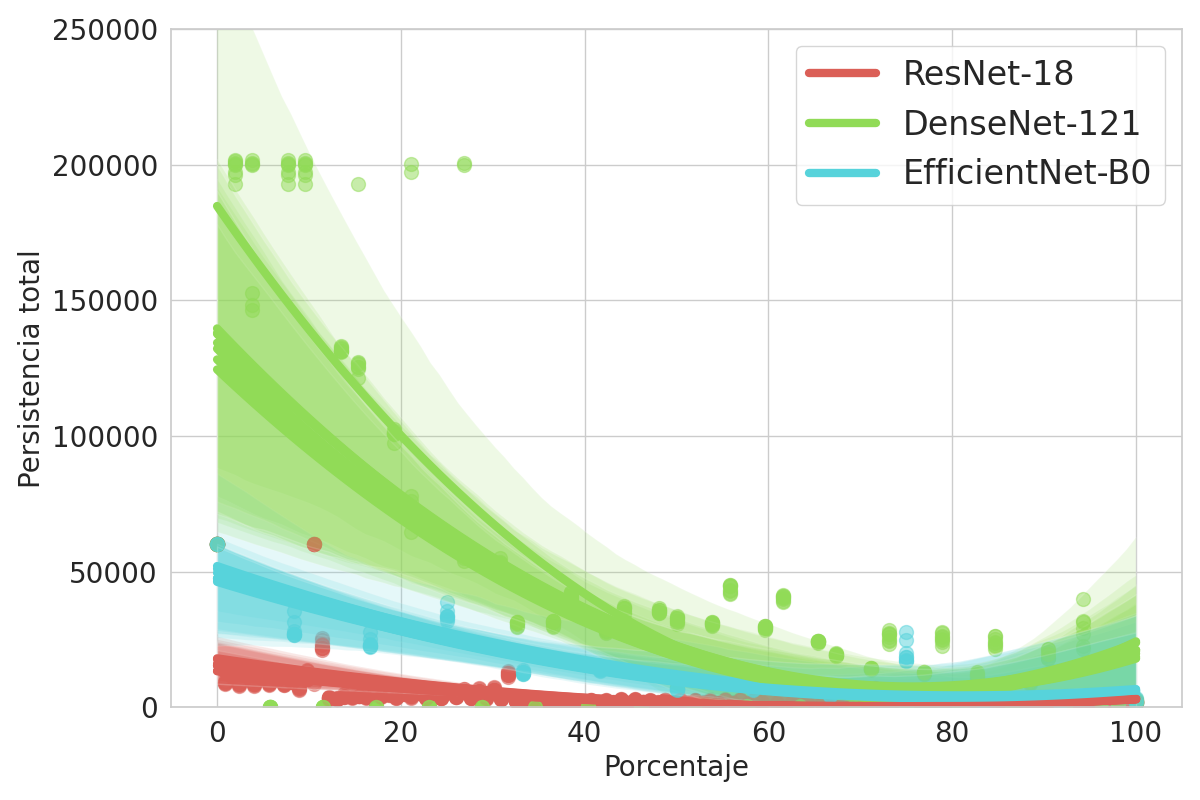
\includegraphics[width=\linewidth]{img/m_arch.png}
		\caption{Persistencia total según el porcentaje de avance en las redes para los modelos ResNet-18, DenseNet-121 y EfficientNet-B0.}
		\label{fig:m-homology-arch-1}
	\end{subfigure}%
	\begin{subfigure}{.5\textwidth}
		\centering
		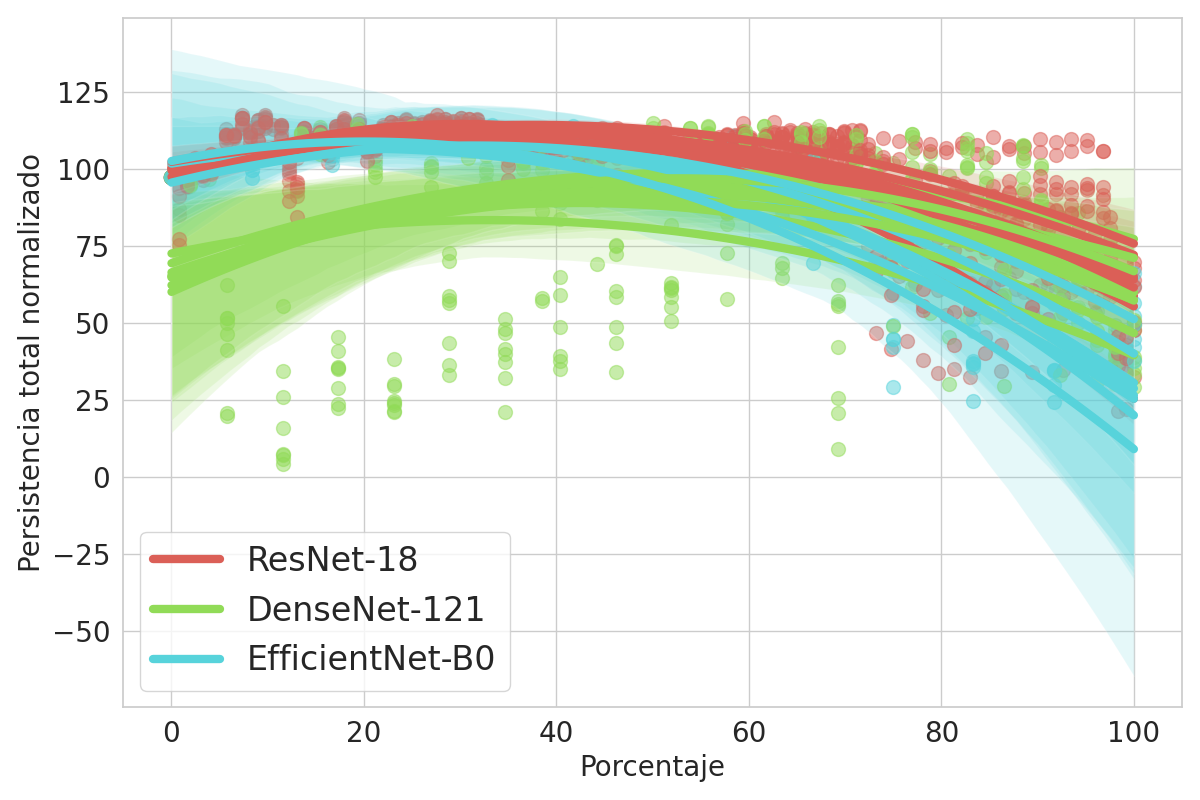
\includegraphics[width=\linewidth]{img/m_arch_norm.png}
		\caption{Persistencia total normalizada según el porcentaje de avance en las redes para los modelos ResNet-18, DenseNet-121 y EfficientNet-B0.}
		\label{fig:m-homology-arch-2}
	\end{subfigure}
	\caption{Comparación de la persistencia total (a) y la persistencia total normalizada (b) de diferentes arquitecturas de redes neuronales en función del porcentaje de avance de los datos a través de la red para la especificidad Marca-Modelo.}
	\label{fig:m-homology-arch}
\end{figure}

\paragraph{Especificidad Marca-Modelo}

Los resultados de las gráficas de la \autoref{fig:mm-homology-arch} muestran una tendencia similar. En este caso, las tendencias del modelo DenseNet-121 en la \autoref{fig:mm-homology-arch-1} muestran una pendiente más pronunciada, indicando transformaciones más agresivas en la homología persistente de los datos. Por otro lado, la \autoref{fig:mm-homology-arch-2} muestra un comportamiento algo diferente respecto a la obtenida en la especificidad Marca, obteniendo unos valores de persistencia total normalizada notablemente superiores al final de las ejecuciones. Dicha consecuencia puede deberse al aumento en la granularidad de la clasificación, haciendo necesarias un mayor número de componentes conexas para facilitar dicha tarea.

\begin{figure}[H]
	\centering
	\begin{subfigure}{.5\textwidth}
		\centering
		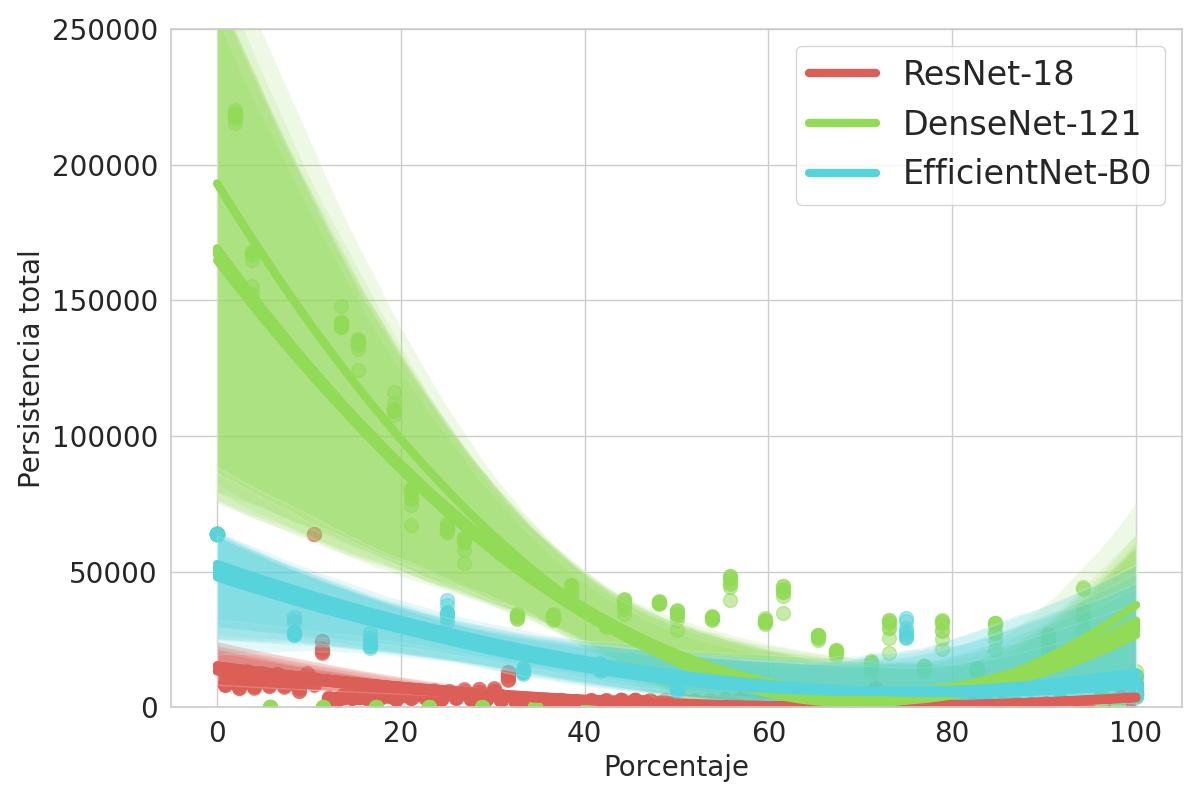
\includegraphics[width=\linewidth]{img/mm_arch.png}
		\caption{Persistencia total según el porcentaje de avance en las redes para los modelos ResNet-18, DenseNet-121 y EfficientNet-B0.}
		\label{fig:mm-homology-arch-1}
	\end{subfigure}%
	\begin{subfigure}{.5\textwidth}
		\centering
		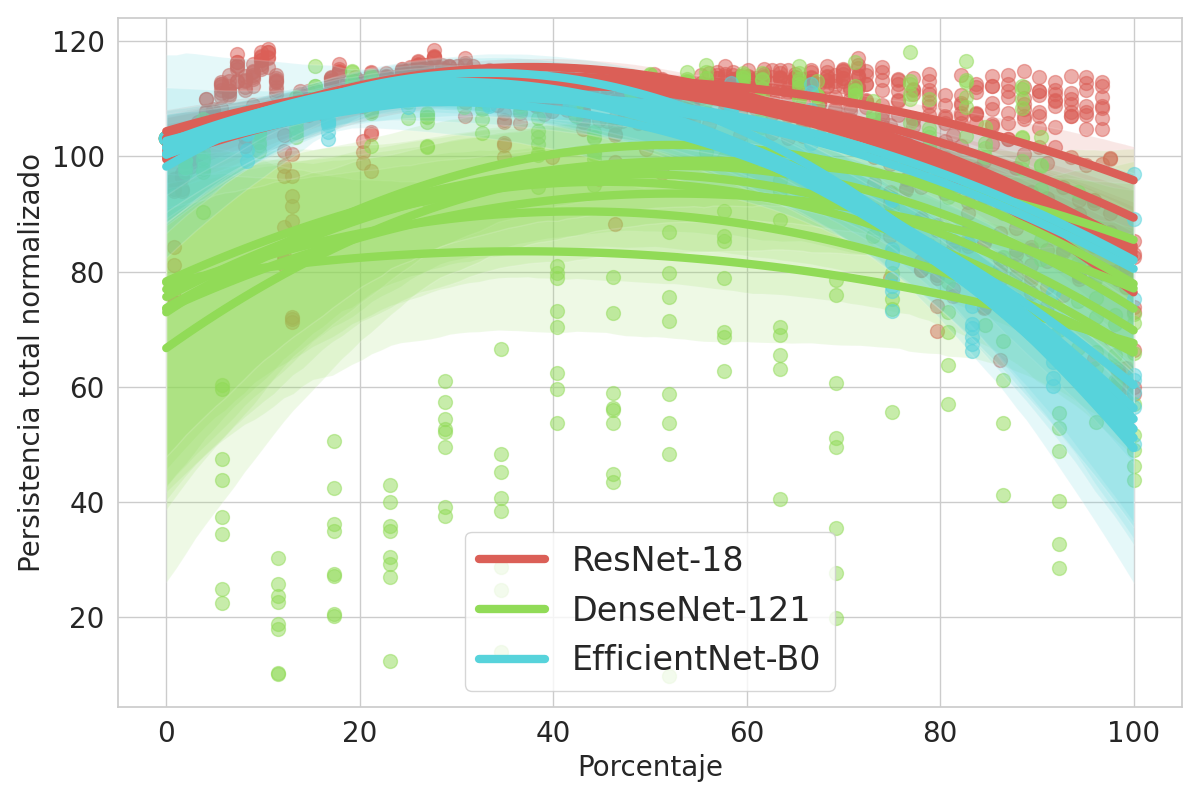
\includegraphics[width=\linewidth]{img/mm_arch_norm.png}
		\caption{Persistencia total normalizada según el porcentaje de avance en las redes para los modelos ResNet-18, DenseNet-121 y EfficientNet-B0.}
		\label{fig:mm-homology-arch-2}
	\end{subfigure}
	\caption{Comparación de la persistencia total (a) y la persistencia total normalizada (b) de diferentes arquitecturas de redes neuronales en función del porcentaje de avance de los datos a través de la red para la especificidad Marca-Modelo.}
	\label{fig:mm-homology-arch}
\end{figure}

Es claro que las Figuras \ref{fig:m-homology-arch} y \ref{fig:mm-homology-arch} indican que la arquitectura escogida es un factor determinante en las transformaciones que los datos sufren desde el punto de vista topológico. Todos los modelos entrenados con la misma arquitectura muestran evoluciones muy similares incluso para las distintas especificidades, donde si que se aprecia un desplazamiento vertical de la homología persistente en función de la granularidad de las clases del conjunto. 

\subsection{Comparación según el optimizador}
\label{subsec:optim}

\paragraph{Especificidad Marca}

A diferencia de la comparativa en función de la arquitectura, la \autoref{fig:m-homology-optim} no muestra patrones tan claros en cómo afecta el optimizador a la persistencia homológica. La \autoref{fig:m-homology-optim-1} muestra cómo los modelos que presentan una menor persistencia total al inicio, como ResNet-18, tienden a presentar una persistencia inicial todavía menor para el optimizador SGD. Sin embargo, esta tendencia empieza a cambiar cuando vamos pasando a modelos de mayor complejidad topológica como DenseNet-121, donde en general Adam parece mostrar una menor persistencia inicial. Por otro lado, la \autoref{fig:m-homology-optim-2} no parece mostrar ningún patrón que nos indique que la elección del optimizador sea relevante para la modificación de la homología persistente de los datos.

\begin{figure}[H]
	\centering
	\begin{subfigure}{.5\textwidth}
		\centering
		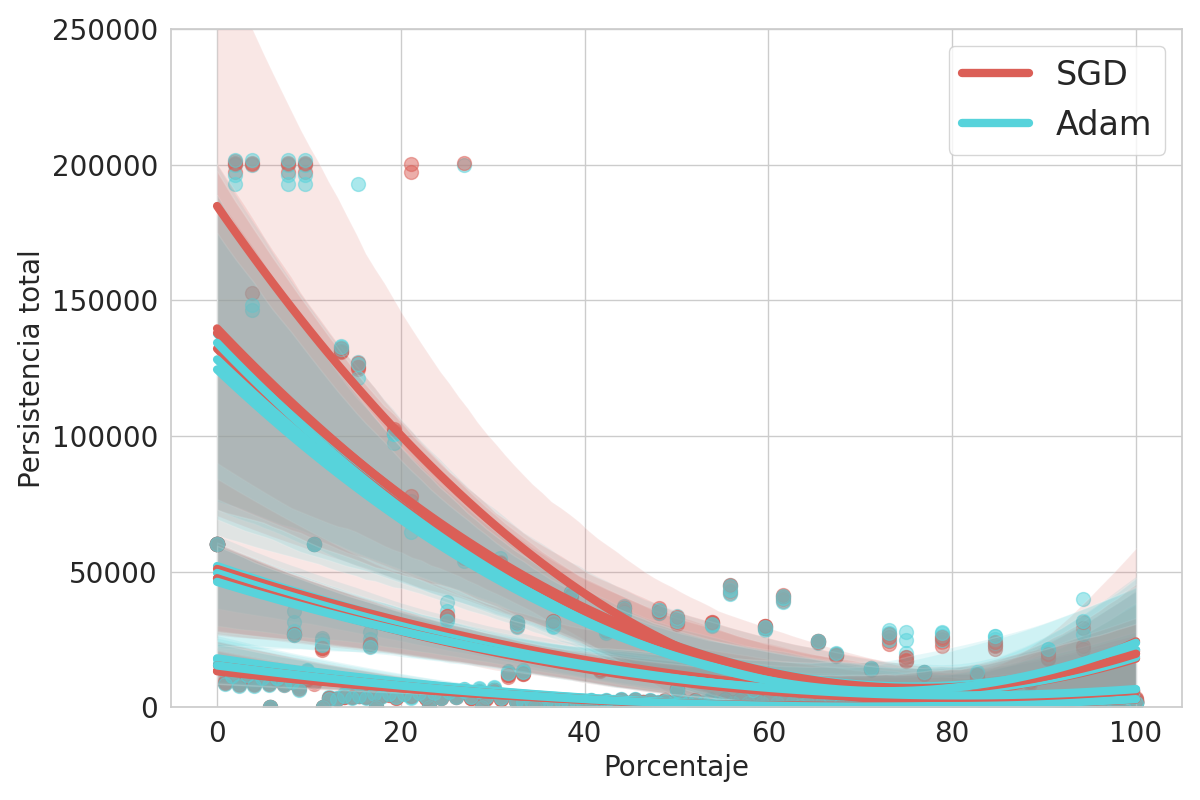
\includegraphics[width=\linewidth]{img/m_optim.png}
		\caption{Persistencia total según el porcentaje de avance en las redes para optimizadores SGD y Adam.}
		\label{fig:m-homology-optim-1}
	\end{subfigure}%
	\begin{subfigure}{.5\textwidth}
		\centering
		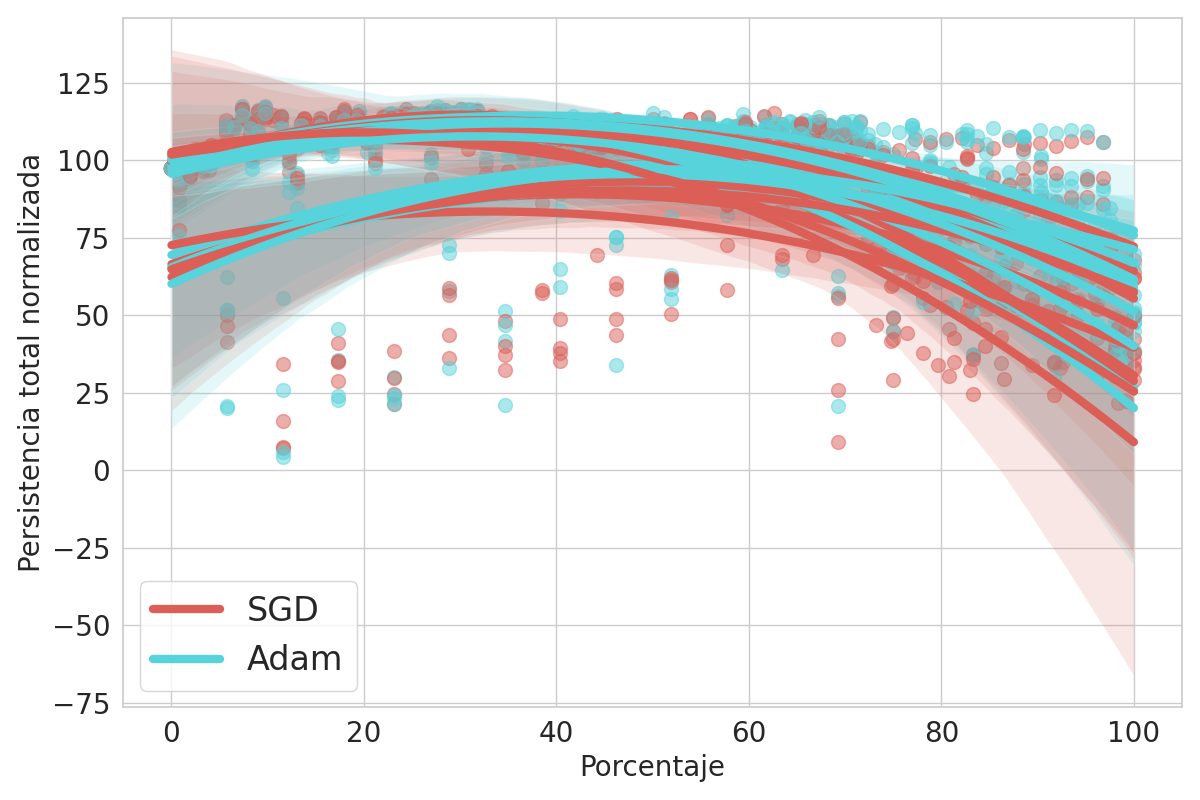
\includegraphics[width=\linewidth]{img/m_optim_norm.png}
		\caption{Persistencia total normalizada según el porcentaje de avance en las redes para SGD y Adam.}
		\label{fig:m-homology-optim-2}
	\end{subfigure}
	\caption{Comparación de la persistencia total (a) y la persistencia total normalizada (b) de diferentes optimizadores de redes neuronales en función del porcentaje de avance de los datos a través de la red para la especificidad Marca.}
	\label{fig:m-homology-optim}
\end{figure}

\paragraph{Especificidad Marca-Modelo}

De nuevo, los resultados obtenidos en la \autoref{fig:mm-homology-optim} son poco esclarecedores acerca de la homología de los datos. No obstante, el aumento en el número de clases parece haber homogeneizado las diferencias observadas en la persistencia total, tal y como muestra la \autoref{fig:mm-homology-optim-1}. Además, las tendencias en la \autoref{fig:mm-homology-optim-2} muestran una mayor persistencia total normalizada al final de la inferencia para los modelos entrenados con Adam.

\begin{figure}[H]
	\centering
	\begin{subfigure}{.5\textwidth}
		\centering
		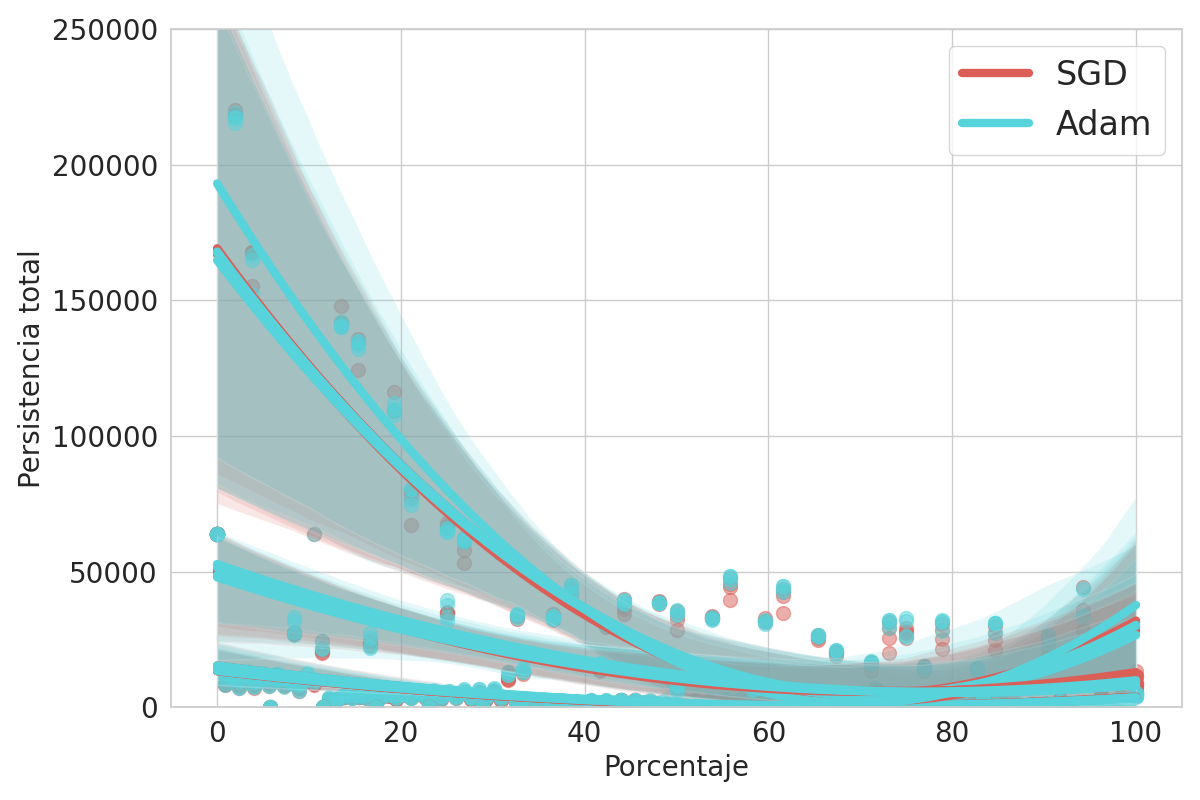
\includegraphics[width=\linewidth]{img/mm_optim.png}
		\caption{Persistencia total normalizada según el porcentaje de avance en la red para optimizadores SGD y Adam.}
		\label{fig:mm-homology-optim-1}
	\end{subfigure}%
	\begin{subfigure}{.5\textwidth}
		\centering
		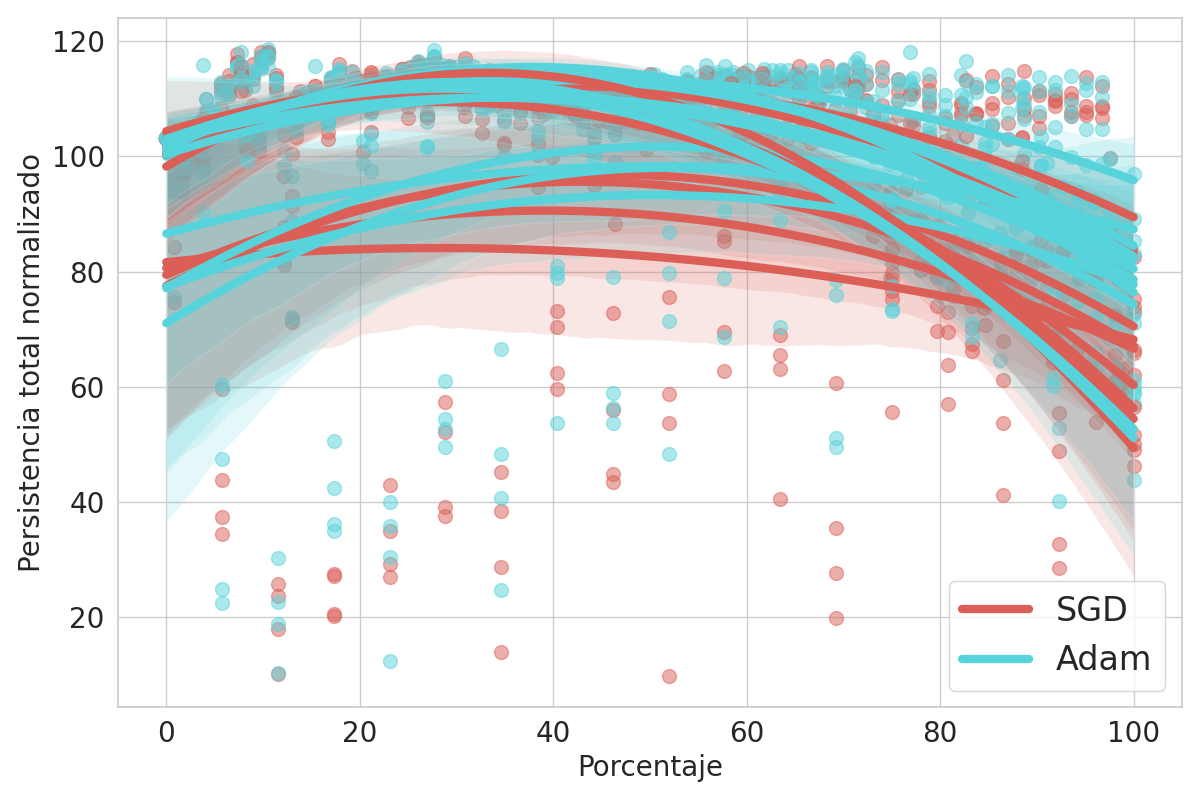
\includegraphics[width=\linewidth]{img/mm_optim_norm.png}
		\caption{Persistencia total normalizada según el porcentaje de avance en la red para optimizadores SGD y Adam.}
		\label{fig:mm-homology-optim-2}
	\end{subfigure}
	\caption{Comparación de la persistencia total (a) y la persistencia total normalizada (b) de diferentes optimizadores de redes neuronales en función del porcentaje de avance de los datos a través de la red para la especificidad Marca-Modelo.}
	\label{fig:mm-homology-optim}
\end{figure}

Los resultados recién vistos sobre las Figuras \ref{fig:m-homology-optim} y \ref{fig:mm-homology-optim} parecen mostrar que el optimizador escogido (al menos, en el caso de los dos empleados) no es un factor especialmente relevante a la hora de modificar la \enquote{forma} de los datos. A pesar de ello, las tendencias observadas al inicio de la red en la persistencia total y al final de ella en la persistencia total normalizada muestran de manera débil ciertos patrones que podrían estudiarse en más profundidad.

\subsection{Comparación según el tamaño de lote}
\label{subsec:batch}

\paragraph{Especificidad Marca}

Las gráficas de la \autoref{fig:m-homology-batch} no muestran ninguna influencia directa o significativa de la elección del tamaño de lote en el ámbito de la topología de los datos durante la etapa de entrenamiento. Las curvas de regresión se muestran muy entrelazadas y las nubes de puntos no muestran claras distinciones o agrupaciones.

\begin{figure}[H]
	\centering
	\begin{subfigure}{.5\textwidth}
		\centering
		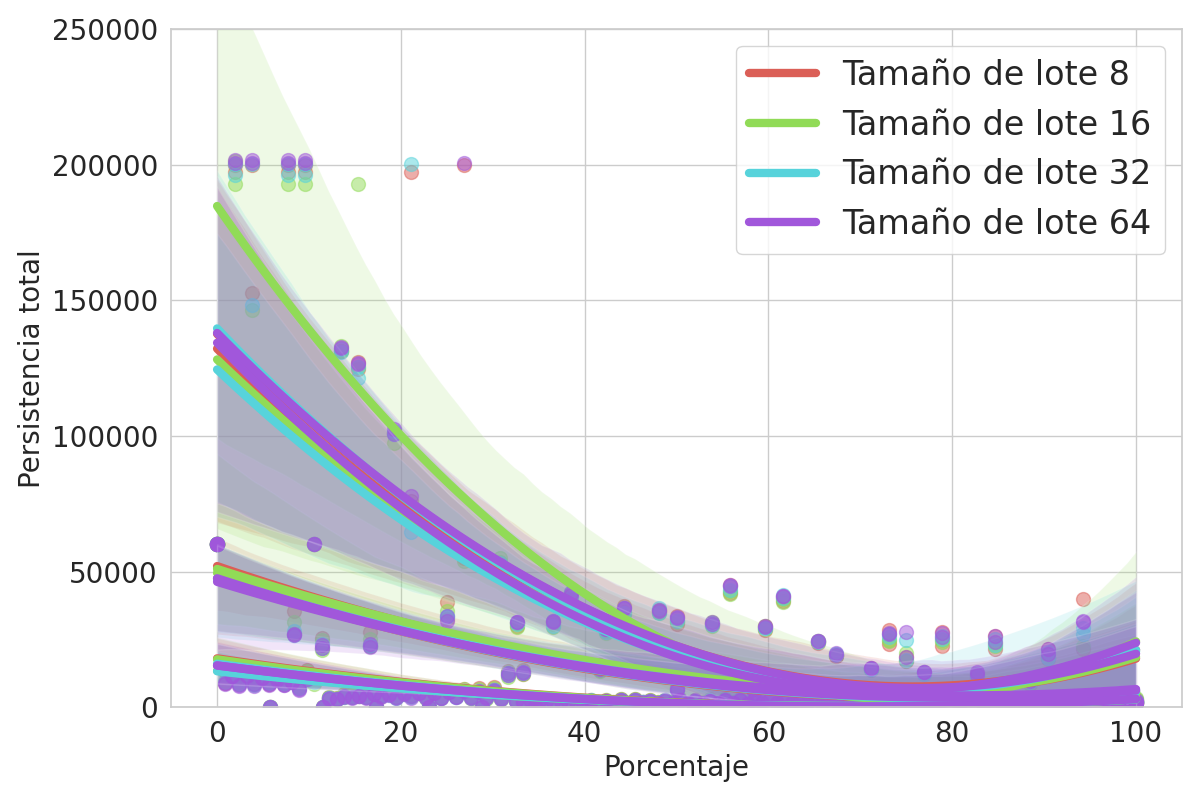
\includegraphics[width=\linewidth]{img/m_batch.png}
		\caption{Persistencia total según el porcentaje de avance en las redes entrenadas para diferentes tamaños de lote.}
		\label{fig:m-homology-batch-1}
	\end{subfigure}%
	\begin{subfigure}{.5\textwidth}
		\centering
		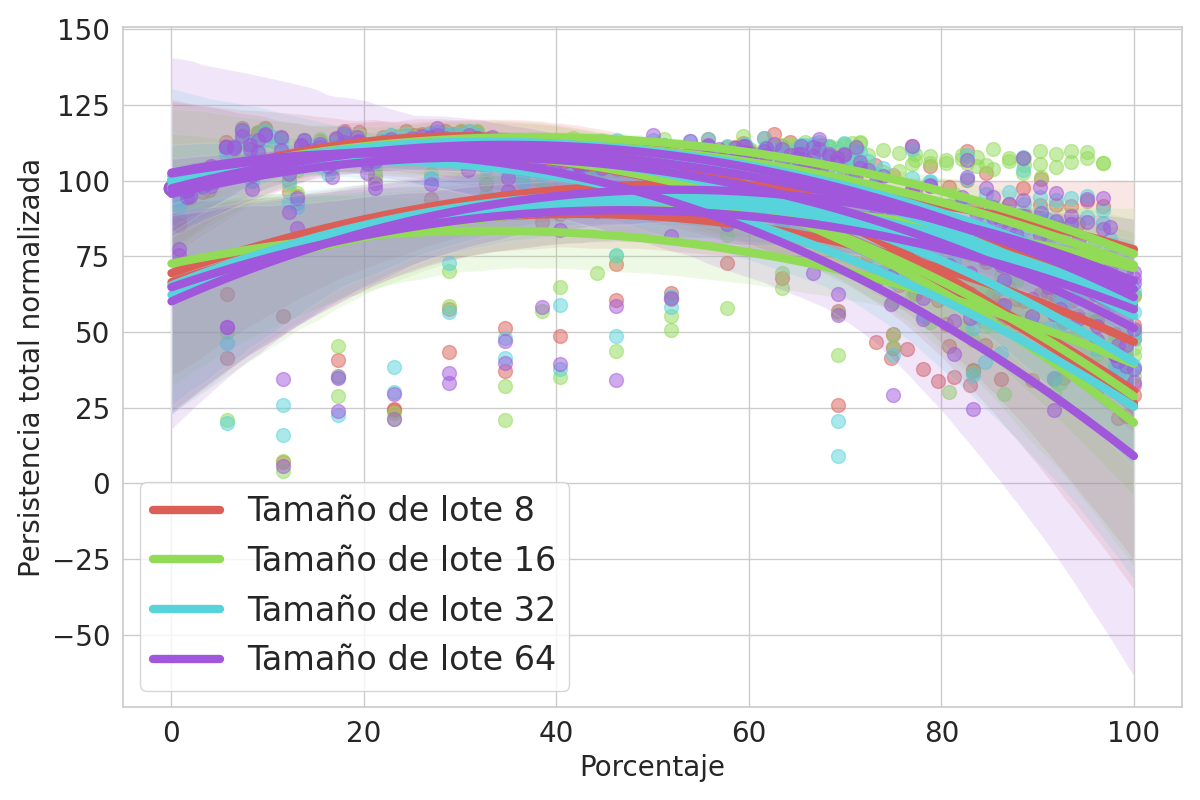
\includegraphics[width=\linewidth]{img/m_batch_norm.png}
		\caption{Persistencia total normalizada según el porcentaje de avance en las redes para diferentes tamaños de lote.}
		\label{fig:m-homology-batch-2}
	\end{subfigure}
	\caption{Comparación de la persistencia total (a) y la persistencia total normalizada (b) para diferentes tamaños de lote en función del porcentaje de avance de los datos a través de la red para la especificidad Marca.}
	\label{fig:m-homology-batch}
\end{figure}

\paragraph{Especificidad Marca-Modelo}

La misma observación se obtiene para los modelos entrenados en la especificidad Marca-Modelo, donde las gráficas de la \autoref{fig:mm-homology-batch} muestran un patrón bastante similar a las recién comentadas.

\begin{figure}[H]
	\centering
	\begin{subfigure}{.5\textwidth}
		\centering
		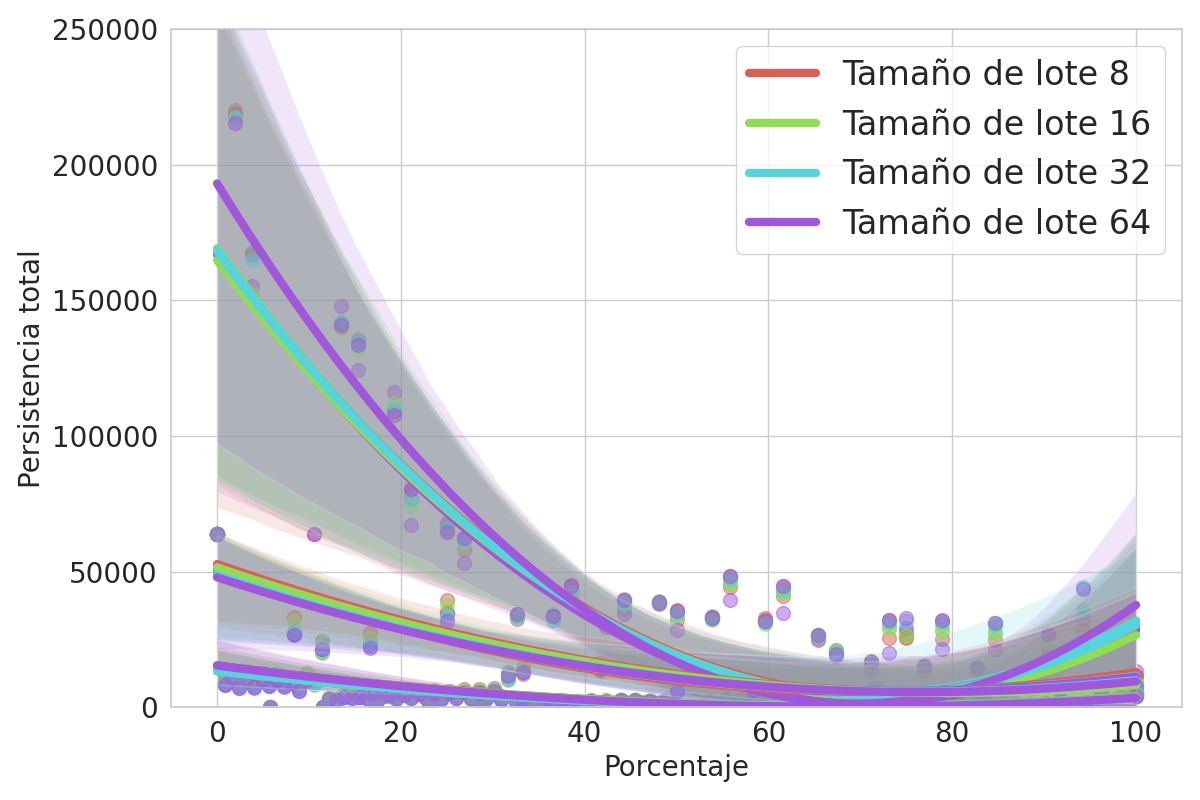
\includegraphics[width=\linewidth]{img/mm_batch.png}
		\caption{Persistencia total según el porcentaje de avance en las redes para diferentes tamaños de lote.}
		\label{fig:mm-homology-batch-1}
	\end{subfigure}%
	\begin{subfigure}{.5\textwidth}
		\centering
		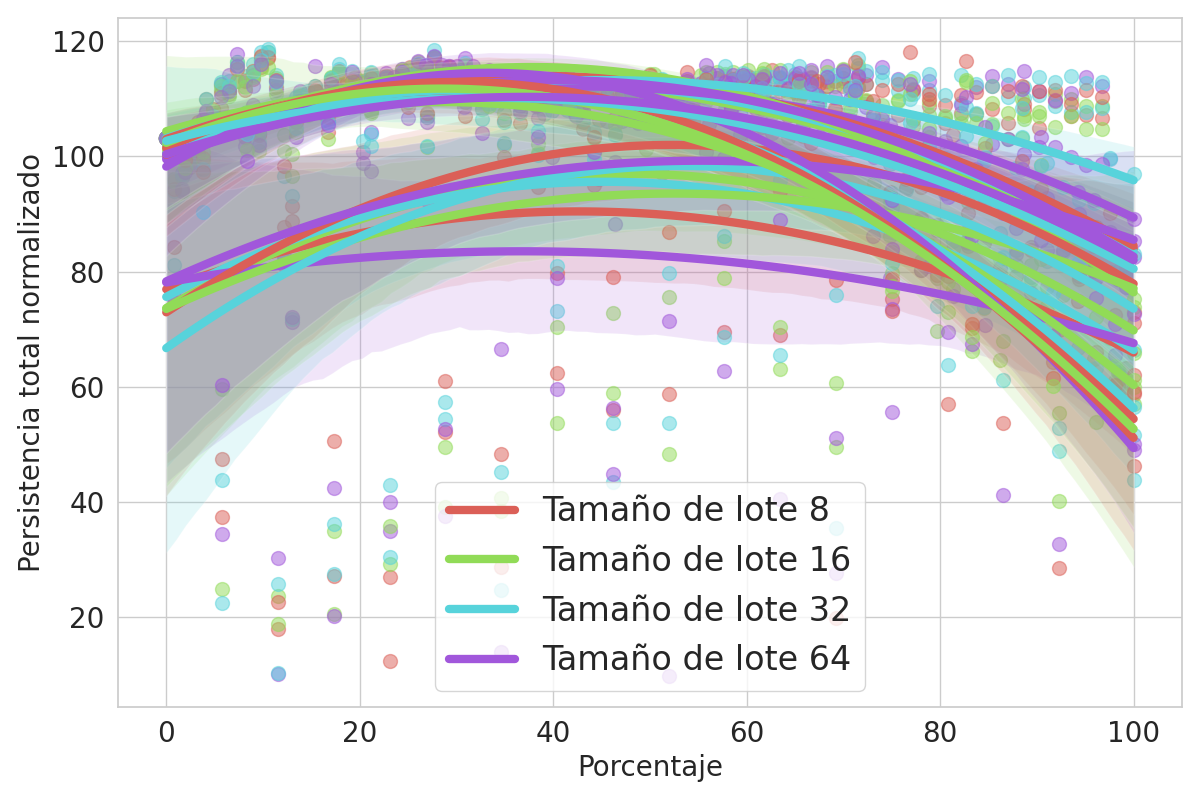
\includegraphics[width=\linewidth]{img/mm_batch_norm.png}
		\caption{Persistencia total normalizada según el porcentaje de avance en las redes para diferentes tamaños de lote.}
		\label{fig:mm-homology-batch-2}
	\end{subfigure}
	\caption{Comparación de la persistencia total (a) y la persistencia total normalizada (b) para diferentes tamaños de lote en función del porcentaje de avance de los datos a través de la red para la especificidad Marca-Modelo.}
	\label{fig:mm-homology-batch}
\end{figure}

Es curioso observar que esta elección de hiperparámetros no muestre alteraciones en la homología persistente de los datos de test estudiados. Este hecho podría implicar que los métodos de optimización empleados son poco sensibles al tamaño de lote escogido a la hora de inferir la variedad subyacente de los datos.

\subsection{Comparación en función del aumento de datos}
\label{subsec:aug}

A continuación trabajaremos sobre los modelos escogidos en la \autoref{subsec:hiperparam} para cada especificidad.

\paragraph{Especificidad Marca: EfficientNet-B0}

La \autoref{fig:m-homology} muestra los resultados de persistencia total y persistencia total normalizada para el modelo base de EfficientNet-B0 y su variante con aumento de datos. Podemos observar que el modelo que obtuvo mejores métricas en el conjunto de test, el modelo base, presenta una persistencia total superior tanto al inicio como al final respecto al modelo con aumento de datos, mientras que es menor en el punto medio de la ejecución, tal y como se ve en la \autoref{fig:m-homology-1}. Esto es, el modelo con mejores métricas muestra transformaciones más agresivas sobre la variedad subyacente de los datos.

En cuanto a la \autoref{fig:m-homology-2}, vemos que el modelo con aumento de datos presenta una persistencia total normalizada inicial más alta que el modelo base y una final más baja. Además, vemos que el máximo de persistencia lo alcanza antes que el modelo base, mostrando una traslación del proceso de aumento de la complejidad en homología persistente a etapas más tempranas de la ejecución.

\begin{figure}[H]
	\centering
	\begin{subfigure}{.5\textwidth}
		\centering
		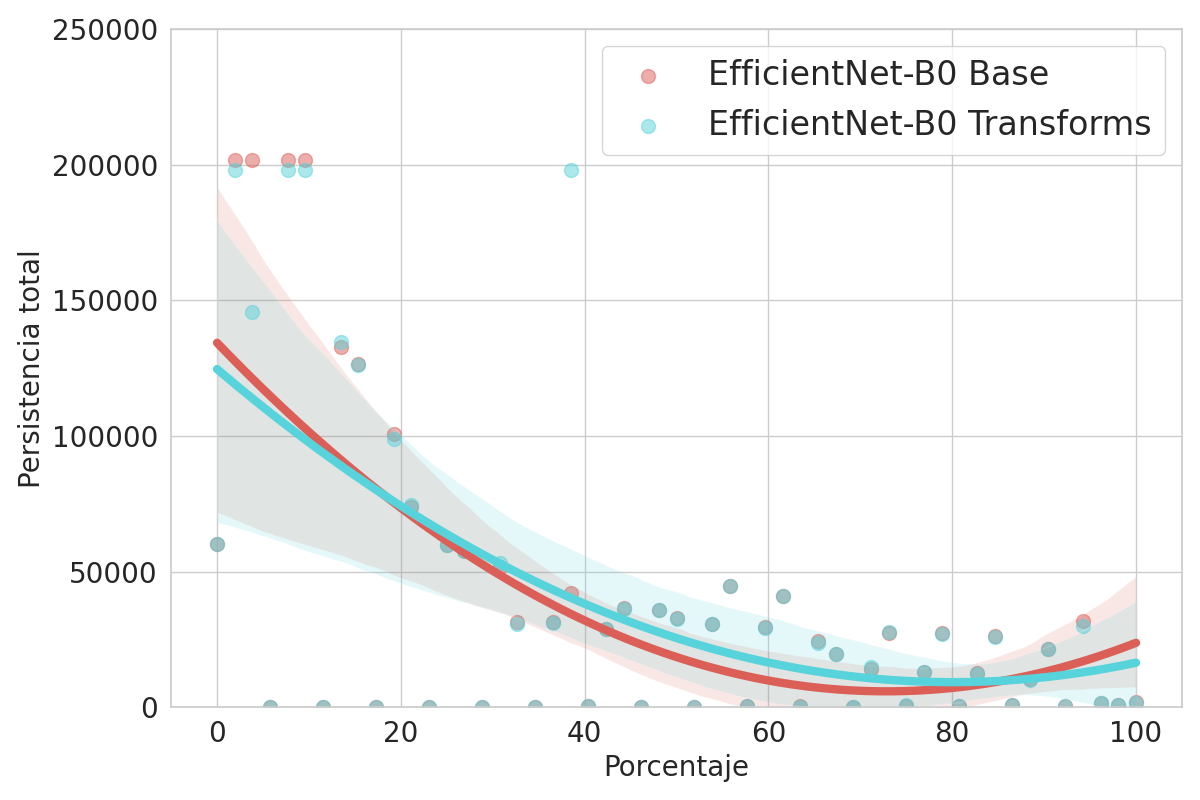
\includegraphics[width=\linewidth]{img/m.png}
		\caption{Persistencia total según el porcentaje de avance en la red para el modelo base entrenado EfficientNet-B0 y su versión con aumento de datos.}
		\label{fig:m-homology-1}
	\end{subfigure}%
	\begin{subfigure}{.5\textwidth}
		\centering
		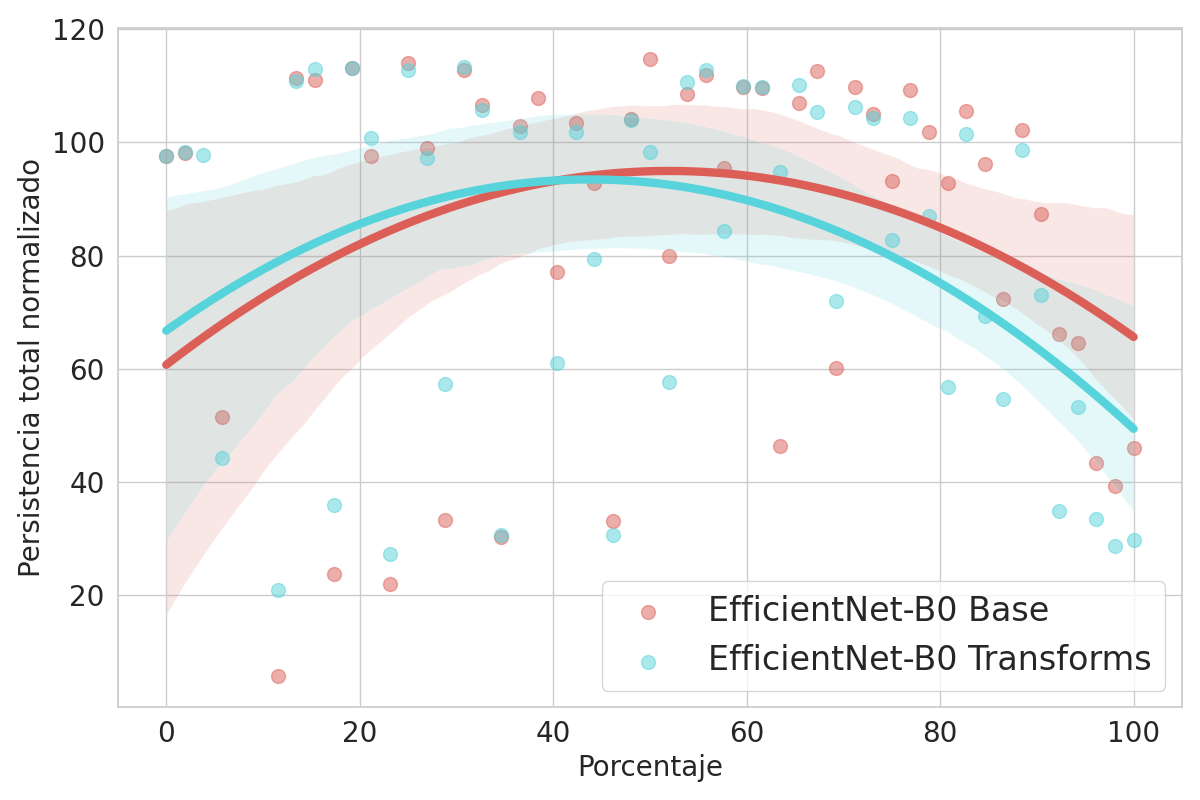
\includegraphics[width=\linewidth]{img/m_norm.png}
		\caption{Persistencia total normalizada según el porcentaje de avance en la red para el modelo base entrenado EfficientNet-B0 y su versión con aumento de datos.}
		\label{fig:m-homology-2}
	\end{subfigure}
	\caption{Comparación de la persistencia total (a) y la persistencia total normalizada (b) para EfficientNet-B0 Base y EfficientNet-B0 Transforms en función del porcentaje de avance de los datos a través de la red para la especificidad Marca.}
	\label{fig:m-homology}
\end{figure}

\paragraph{Especificidad Marca-Modelo: DenseNet-121}

Estas observaciones se ven reforzadas en la \autoref{fig:mm-homology}. En particular, la \autoref{fig:mm-homology-1} muestra dichas observaciones de una manera más agresiva. Vemos que el mejor modelo, DenseNet-121 con aumento de datos, muestra una persistencia total mayor al inicio de la red y al final. Además, la \autoref{fig:mm-homology-2} muestra como el aumento de datos traslada de nuevo el máximo a momentos más tempranos de ejecución y una fuerte reducción de la complejidad total normalizada al final de la red.

\begin{figure}[H]
	\centering
	\begin{subfigure}{.5\textwidth}
		\centering
		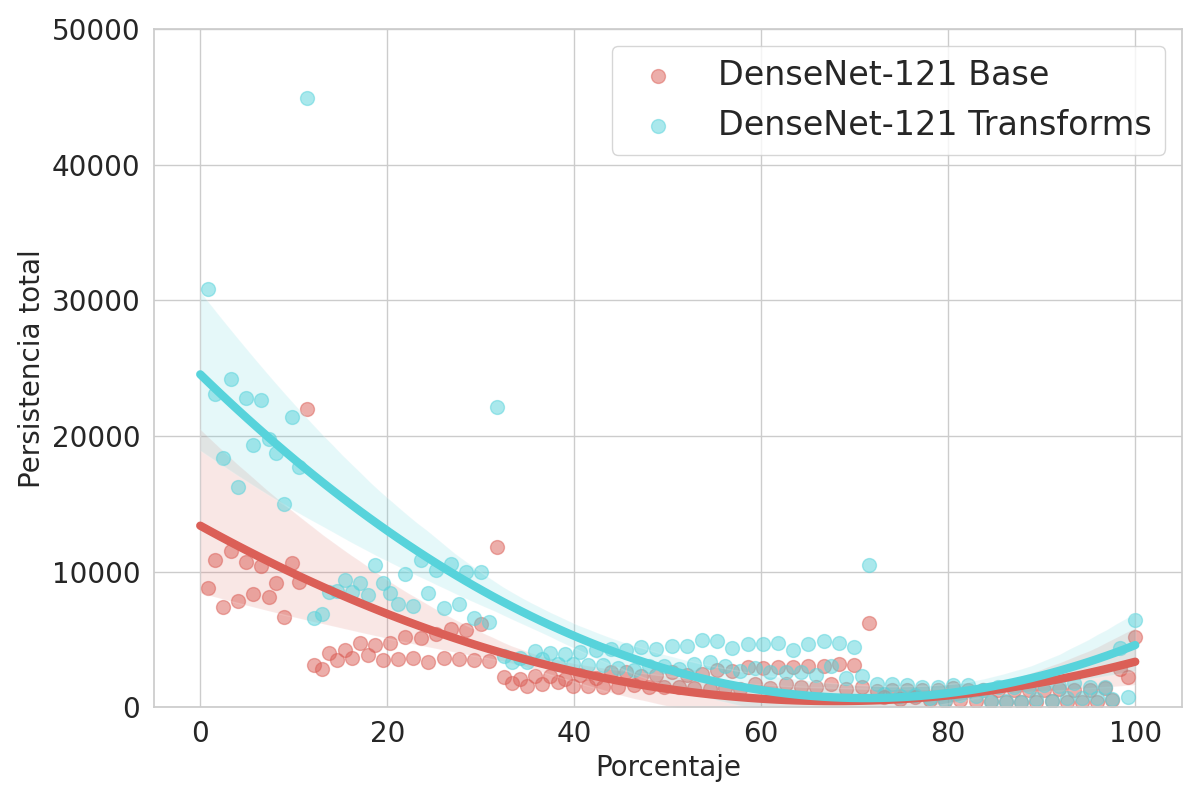
\includegraphics[width=\linewidth]{img/mm.png}
		\caption{Persistencia total según el porcentaje de avance en la red para el modelo base entrenado EfficientNet-B0 y su versión con aumento de datos.}
		\label{fig:mm-homology-1}
	\end{subfigure}%
	\begin{subfigure}{.5\textwidth}
		\centering
		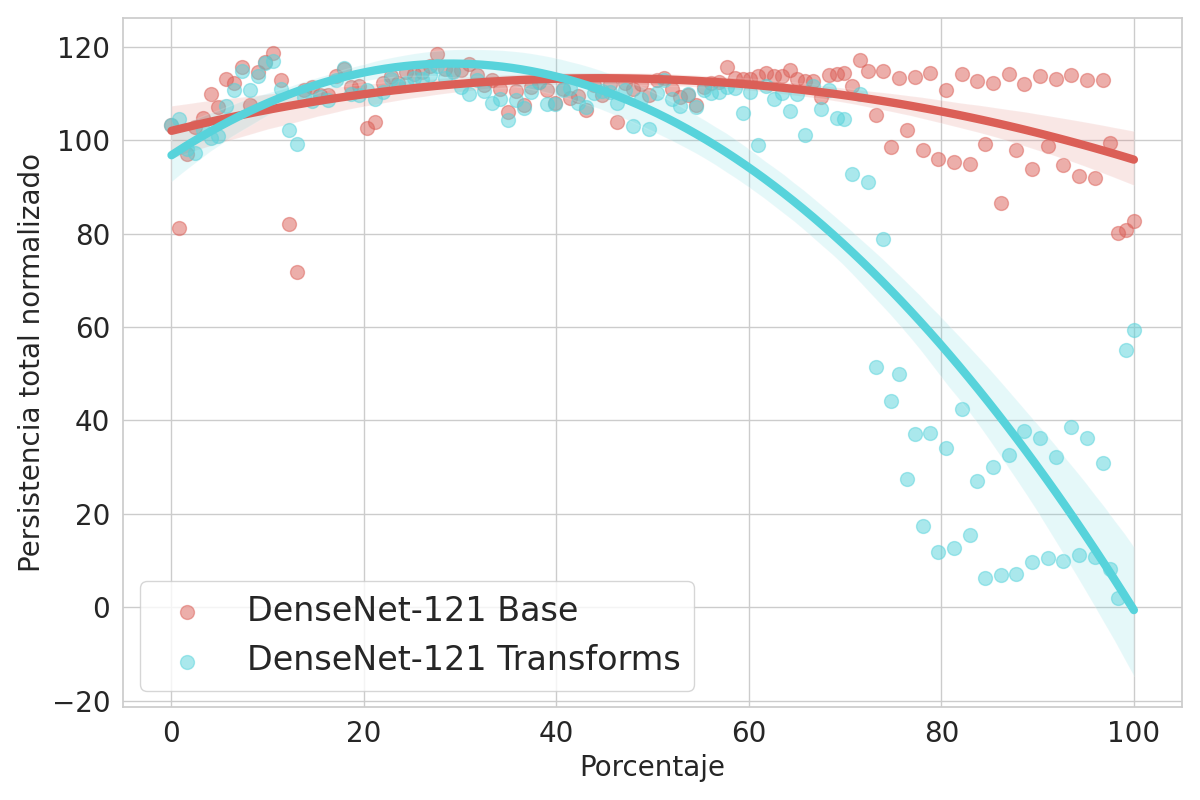
\includegraphics[width=\linewidth]{img/mm_norm.png}
		\caption{Persistencia total normalizada según el porcentaje de avance en la red para el modelo base entrenado EfficientNet-B0 y su versión con aumento de datos.}
		\label{fig:mm-homology-2}
	\end{subfigure}
	\caption{Comparación de la persistencia total (a) y la persistencia total normalizada (b) para EfficientNet-B0 Base y EfficientNet-B0 Transforms en función del porcentaje de avance de los datos a través de la red para la especificidad Marca-Modelo.}
	\label{fig:mm-homology}
\end{figure}

Los resultados recién vistos muestran patrones interesantes en el comportamiento del modelo cuando realizamos aumento de datos: tiende a realizar modificaciones más intensas en fases anteriores de la red y simplificar las estructuras al final del modelo. Este comportamiento muestra que las componentes conexas al final de la red son más compactas y están mejor definidas, lo que lleva a una reducción de la complejidad topológica. No solo eso, si no que al tener en cuenta las clases de persistencia homológicas de dimensión 1, también se reducen el número de componentes conexas que forman bucles, lo que evita entrelazamientos entre éstas.

\subsection{Comparación según la granularidad de las clases}
\label{subsec:grano}

\paragraph{EfficientNet-B0}

EfficientNet-B0 ha mostrado el mejor rendimiento en las métricas empleadas para la especificidad Marca. La persistencia total del modelo entrenado en Marca-Modelo en la \autoref{fig:efficientnet-1} muestra transformaciones más agresivas en la homología persistente de los datos. Aquí, en los extremos de la ejecución los datos presentan una persistencia total más alta y un mínimo inferior al del modelo entrenado para Marca.

Por su parte, la persistencia total normalizada muestra valores regularmente superiores para la especificidad Marca-Modelo a los de Marca (\autoref{fig:efficientnet-2}). Estos hechos parecen coherentes, pues a pesar de corresponderse con el mismo conjunto de datos, la necesidad de etiquetar una mayor variedad de clases implica un desglose más fino de las características de los datos y en consecuencia, una complejidad topológica mayor.

\begin{figure}[H]
	\centering
	\begin{subfigure}{.5\textwidth}
		\centering
		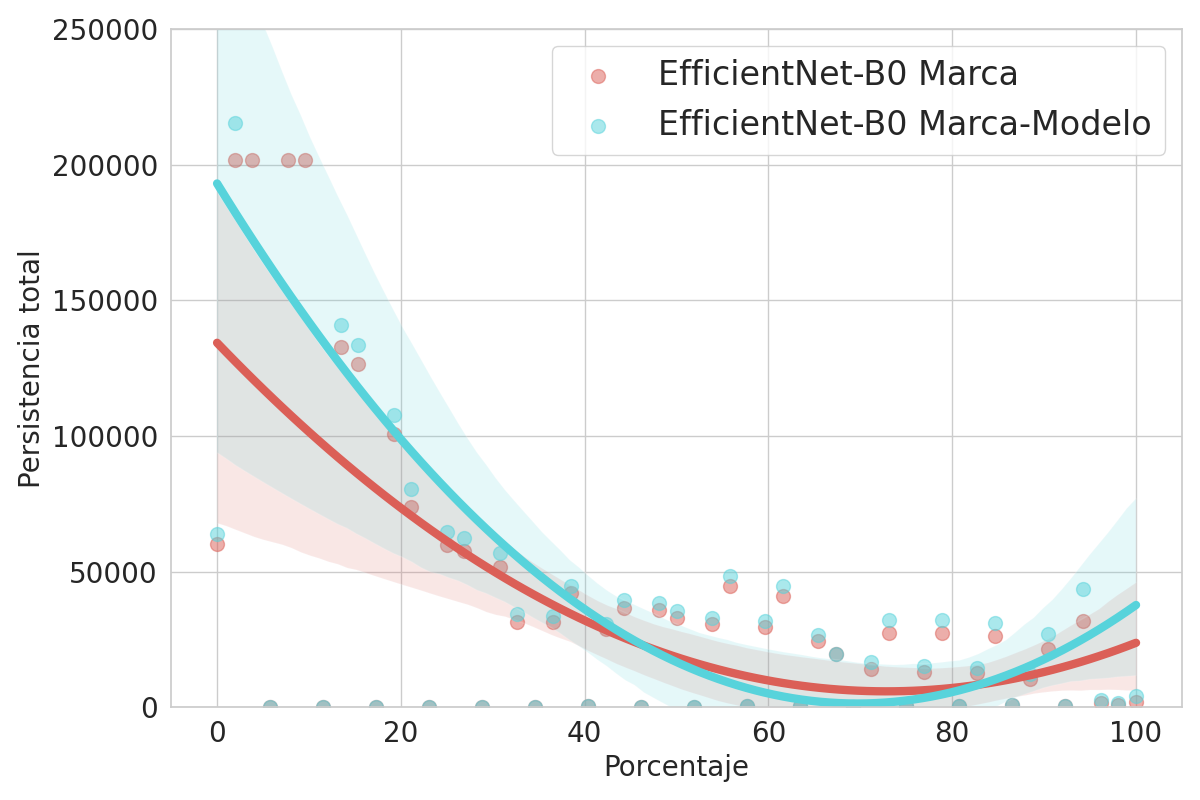
\includegraphics[width=\linewidth]{img/general_efficientnet.png}
		\caption{Persistencia total según el porcentaje de avance en la red para el modelo EfficientNet-B0 entrenado para las especificidades Marca y Marca-Modelo.}
		\label{fig:efficientnet-1}
	\end{subfigure}%
	\begin{subfigure}{.5\textwidth}
		\centering
		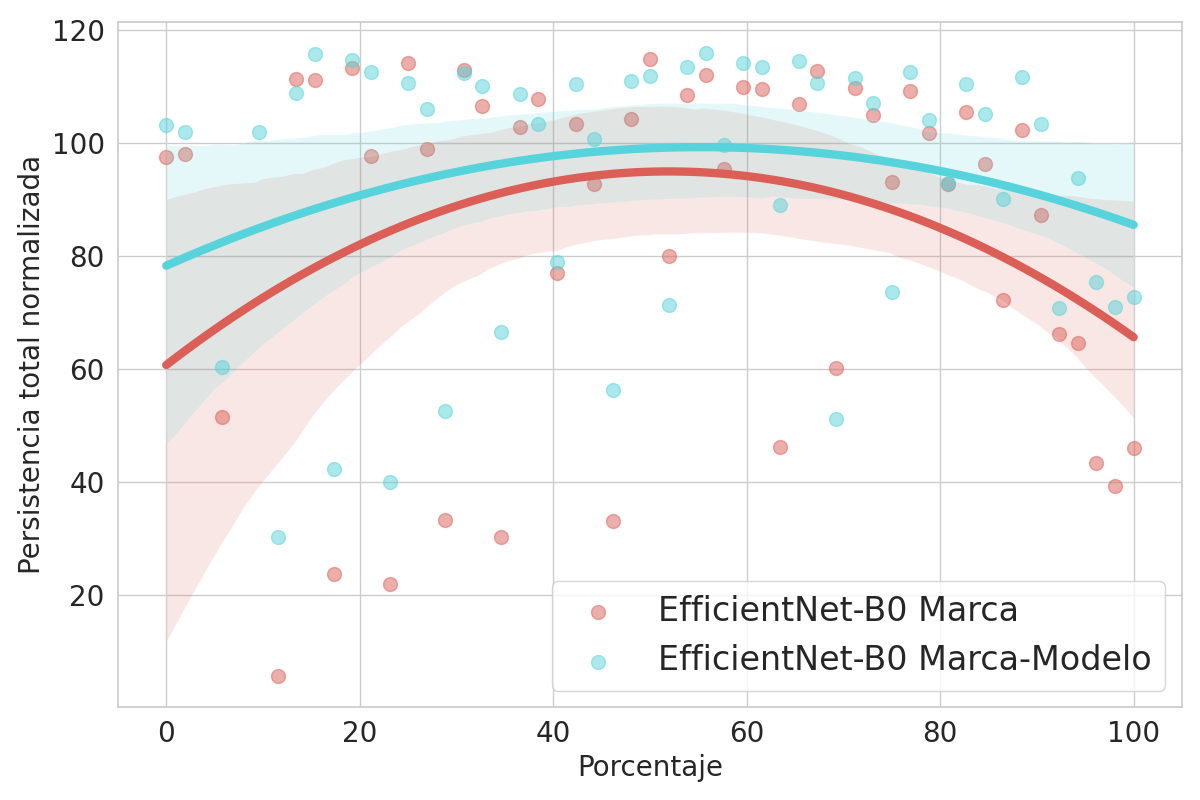
\includegraphics[width=\linewidth]{img/general_efficientnet_norm.png}
		\caption{Persistencia total normalizada según el porcentaje de avance en la red para el modelo EfficientNet-B0 entrenado para las especificidades Marca y Marca-Modelo.}
		\label{fig:efficientnet-2}
	\end{subfigure}
	\caption{Comparación de la persistencia total (a) y la persistencia total normalizada (b) para EfficientNet-B0 entrenado con SGD y un tamaño de lote 64 en función del porcentaje de avance de los datos a través de la red para las especificidades Marca y Marca-Modelo.}
	\label{fig:efficientnet}
\end{figure}

\paragraph{DenseNet-121}

En cuanto a DenseNet-121, vemos en la \autoref{fig:densenet-1} que ambas curvas se asemejan más que en el caso anterior. Es interesante ver como en el último instante de la red, el modelo entrenado para la especificidad Marca-Modelo presenta una subida de persistencia considerable, mientras que la de Marca es más modesta. Este hecho muestra claramente la necesidad del modelo de deshacer la simplificación realizada con el fin de separar los datos para la clasificación.

Además, las muestras tomadas en los distintos instantes de la red muestran cuatro puntos con un aumento considerable de la persistencia total. Estos instantes coinciden con los puntos donde se encuentran las activaciones de transición entre los cuatro bloques densos que presenta DenseNet-121, mostrando cómo las conexiones residuales entre dichos bloques aumenta la complejidad topológica de los datos.

Por otro lado, la \autoref{fig:densenet-2} nos muestra cómo, de nuevo, la persistencia total normalizada presenta en general valores inferiores para la especificidad Marca. Otra observación relevante es la reducción de complejidad más progresiva y gradual que muestra el modelo de Marca en la segunda mitad de la inferencia. El hecho de que DenseNet-121 entrenado con una mayor granularidad requiera de mayor persistencia durante más tiempo puede deberse a la clara dificultad añadida por el aumento de clases.

\begin{figure}[H]
	\centering
	\begin{subfigure}{.5\textwidth}
		\centering
		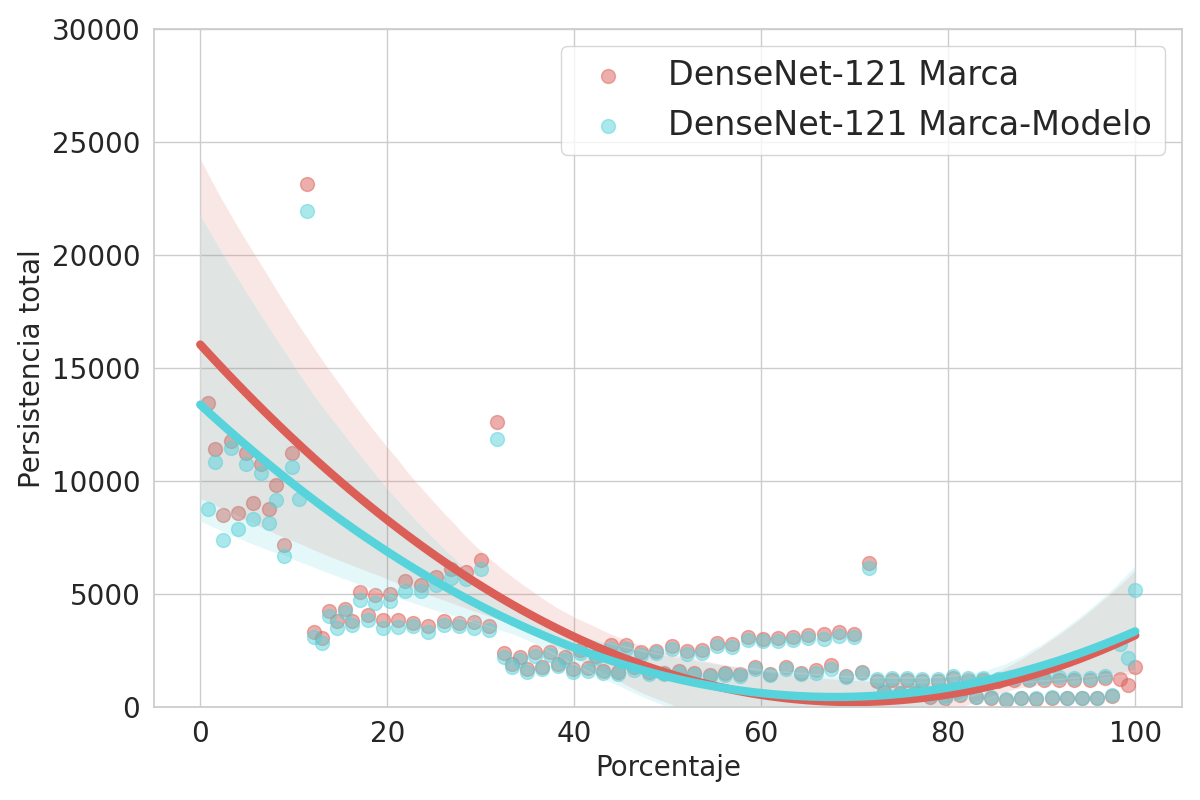
\includegraphics[width=\linewidth]{img/general_densenet.png}
		\caption{Persistencia total según el porcentaje de avance en la red para el modelo DenseNet-121  entrenado para las especificidades Marca y Marca-Modelo.}
		\label{fig:densenet-1}
	\end{subfigure}%
	\begin{subfigure}{.5\textwidth}
		\centering
		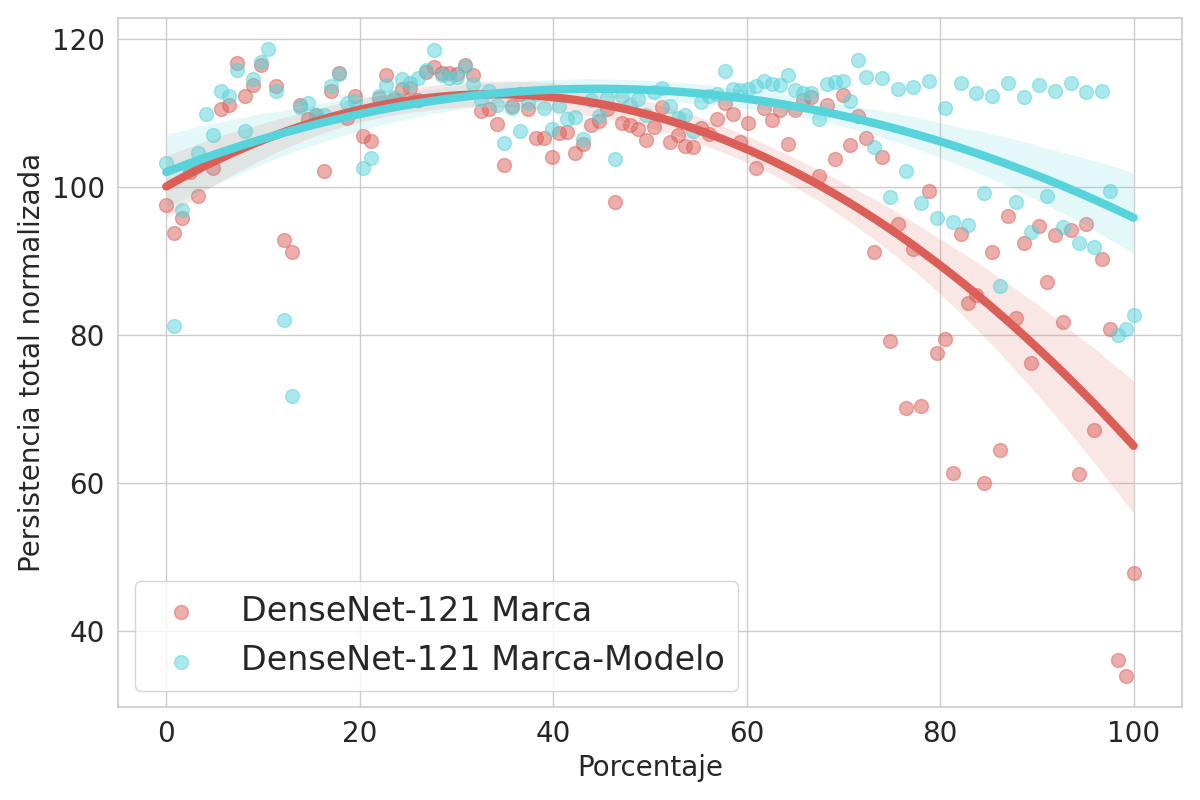
\includegraphics[width=\linewidth]{img/general_densenet_norm.png}
		\caption{Persistencia total normalizada según el porcentaje de avance en la red para el modelo DenseNet-121  entrenado para las especificidades Marca y Marca-Modelo.}
		\label{fig:densenet-2}
	\end{subfigure}
	\caption{Comparación de la persistencia total (a) y la persistencia total normalizada (b) para DenseNet-121 entrenado con SGD y un tamaño de lote 32 en función del porcentaje de avance de los datos a través de la red para las especificidades Marca y Marca-Modelo.}
	\label{fig:densenet}
\end{figure}

\subsection{Comparación según el subconjunto de datos}
\label{subsec:set}

Hasta ahora hemos estado viendo como distintos modelos con distintos hiperparámetros y granularidad durante la etapa de entrenamiento afectan a la variedad subyacente de los datos empleados. A continuación, compararemos cómo transforma un mismo modelo los propios datos en función del subconjunto al que pertenecen: entrenamiento, validación y test.

\paragraph{Especificidad Marca: EfficientNet-B0}

Lo primero que observamos en las Figuras \ref{fig:m_set_base} y \ref{fig:m_set_trans} es una mayor persistencia total al inicio sobre el conjunto de entrenamiento respecto al de validación y test en ambos modelos. Por otro lado, en la \autoref{fig:m_set_base}, que muestra los resultados con mejores métricas, los conjuntos de validación y test muestran una persistencia total prácticamente idéntica, mientras que el modelo con aumento de datos presenta mayores discrepancias al respecto.

Por lo que se refiere a la persistencia total normalizada (Figuras \ref{fig:m_set_base_norm} y \ref{fig:m_set_trans_norm}), observamos tendencias muy similares, donde las curvas de validación y test muestran un ajuste más fino al de entrenamiento para el modelo base que para el modelo con aumento de datos. 

\begin{figure}[H]
	\centering
	\begin{subfigure}{.45\textwidth}
		\centering
		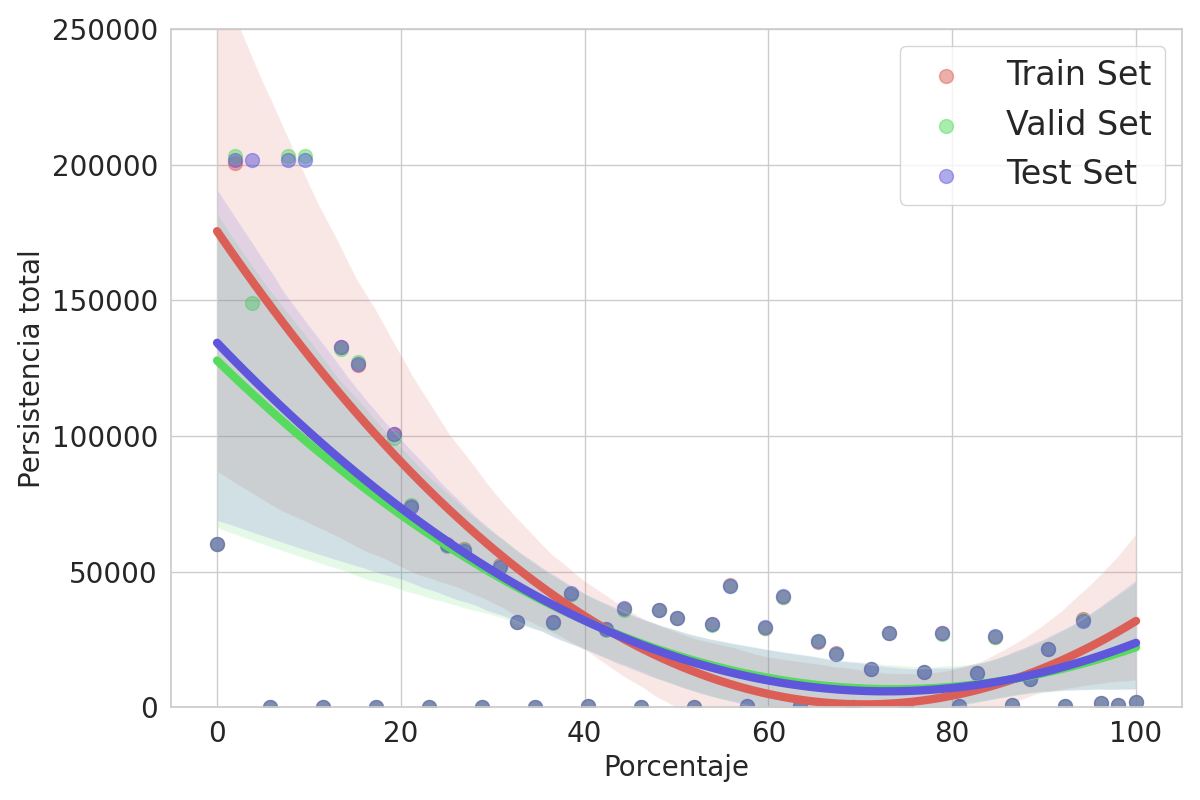
\includegraphics[width=\linewidth]{img/m_set_base.png}
		\caption{Persistencia total según el porcentaje de avance en la red para los conjuntos de entrenamiento, validación y test.}
		\label{fig:m_set_base}
	\end{subfigure}
	\begin{subfigure}{.45\textwidth}
		\centering
		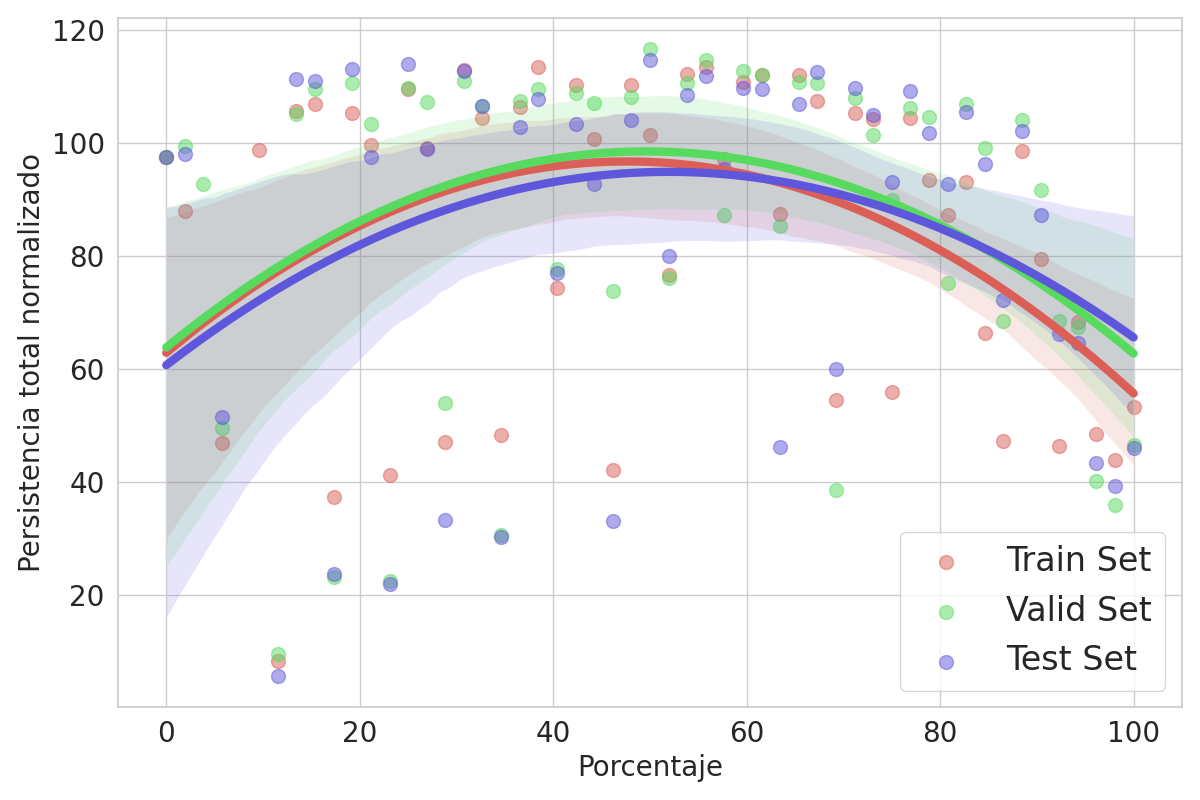
\includegraphics[width=\linewidth]{img/m_set_base_norm.png}
		\caption{Persistencia total normalizada según el porcentaje de avance en la red para los conjuntos de entrenamiento, validación y test.}
		\label{fig:m_set_base_norm}
	\end{subfigure}
	\begin{subfigure}{.45\textwidth}
		\centering
		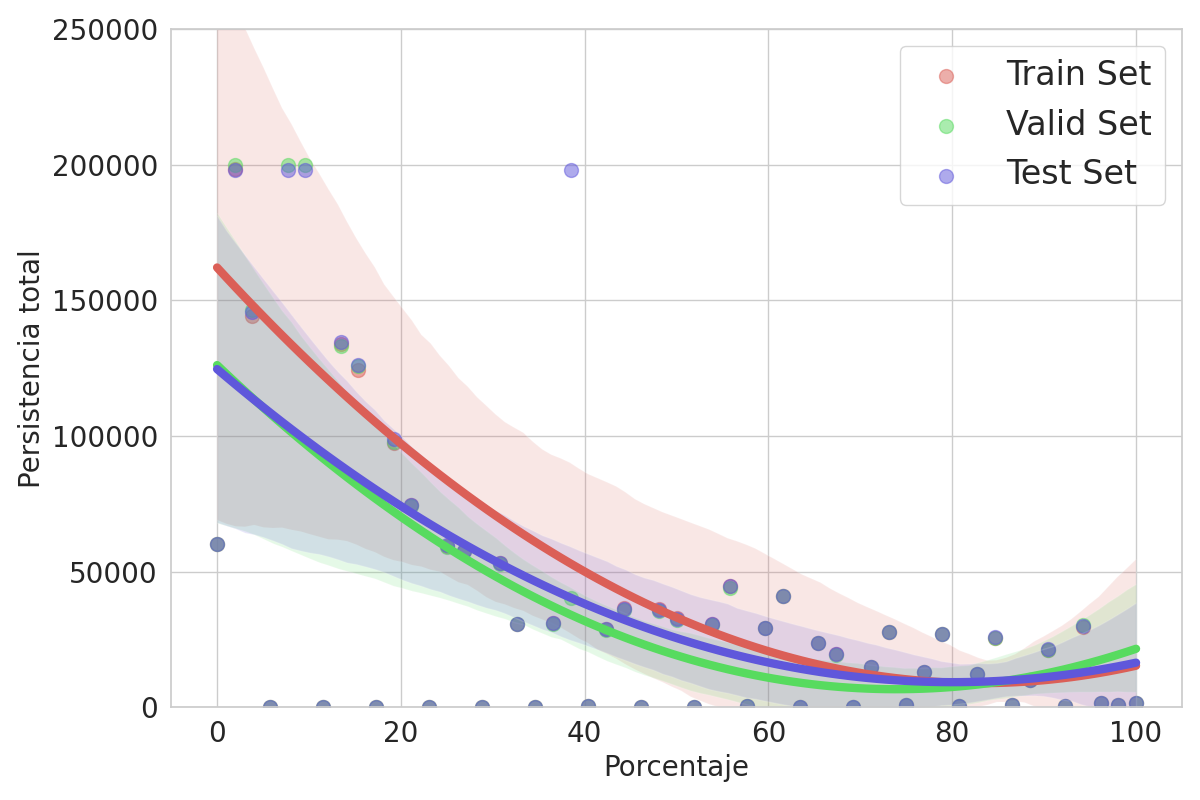
\includegraphics[width=\linewidth]{img/m_set_trans.png}
		\caption{Persistencia total según el porcentaje de avance en la red con aumento de datos para los conjuntos de entrenamiento, validación y test.}
		\label{fig:m_set_trans}
	\end{subfigure}%
	\begin{subfigure}{.45\textwidth}
		\centering
		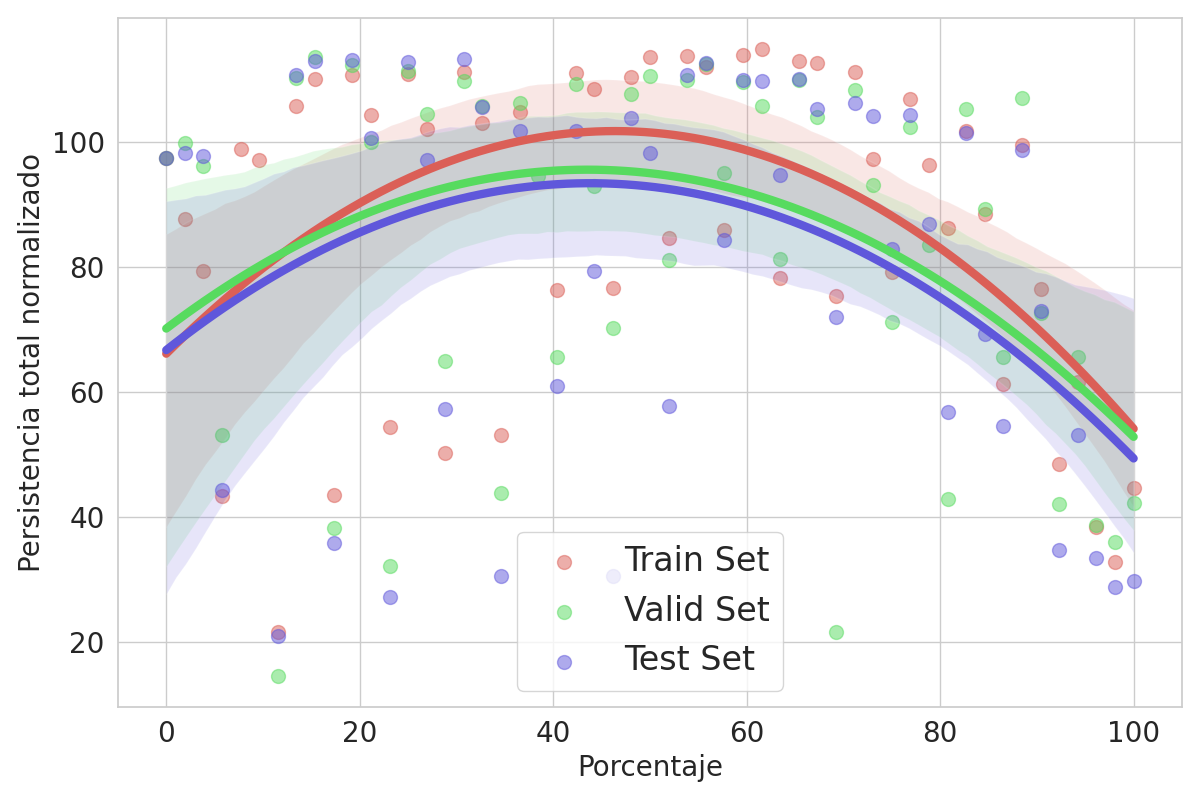
\includegraphics[width=\linewidth]{img/m_set_trans_norm.png}
		\caption{Persistencia total normalizada según el porcentaje de avance en la red con aumento de datos para los conjuntos de entrenamiento, validación y test.}
		\label{fig:m_set_trans_norm}
	\end{subfigure}
	\caption{Comparación de la persistencia total (a, c) y la persistencia total normalizada (b, d) para los conjuntos de entrenamiento, validación y test para la especificidad Marca. Las Subfiguras (a) y (c) representan el modelo base, mientras que las Subfiguras (b) y (d) representan el modelo con aumento de datos.}
	\label{fig:m-set}
\end{figure}

\paragraph{Especificidad Marca-Modelo: DenseNet-121}

Las Figuras \ref{fig:mm_set_base} y \ref{fig:mm_set_trans} muestran un ajuste de la persistencia total prácticamente perfecto entre los tres subconjuntos de datos. Más aún, podemos ver cómo el modelo que ha presentado mejores métricas en el conjunto de test, es decir, el modelo con aumento de datos, presenta un ajuste mucho más fino entre los valores de persistencia total normalizados para los tres subconjuntos (\autoref{fig:mm_set_trans_norm}). Es interesante observar como en esta ocasión, los puntos obtenidos se comportan de manera más homogénea independientemente del subconjunto escogido, a diferencia de lo observado en la \autoref{fig:mm_set_base_norm}.

\begin{figure}[H]
	\centering
	\begin{subfigure}{.45\textwidth}
		\centering
		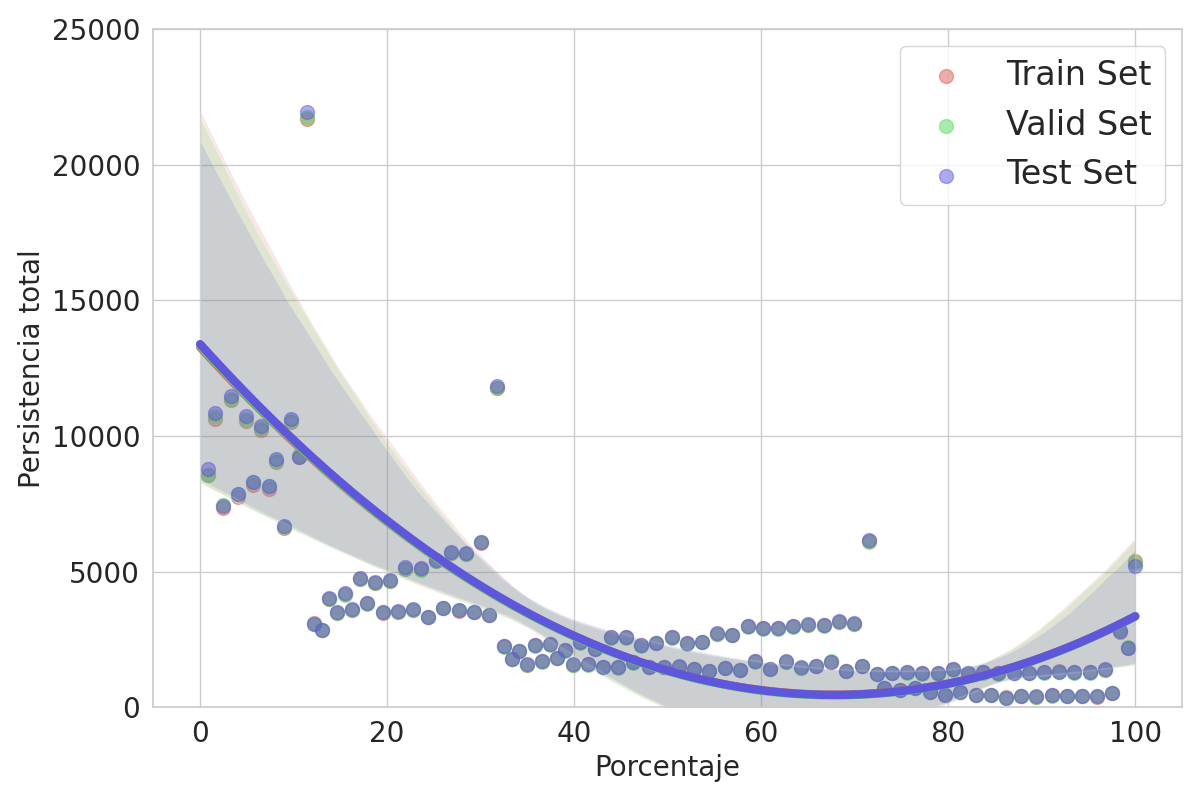
\includegraphics[width=\linewidth]{img/mm_set_base.png}
		\caption{Persistencia total según el porcentaje de avance en la red para los conjuntos de entrenamiento, validación y test.}
		\label{fig:mm_set_base}
	\end{subfigure}
	\begin{subfigure}{.45\textwidth}
		\centering
		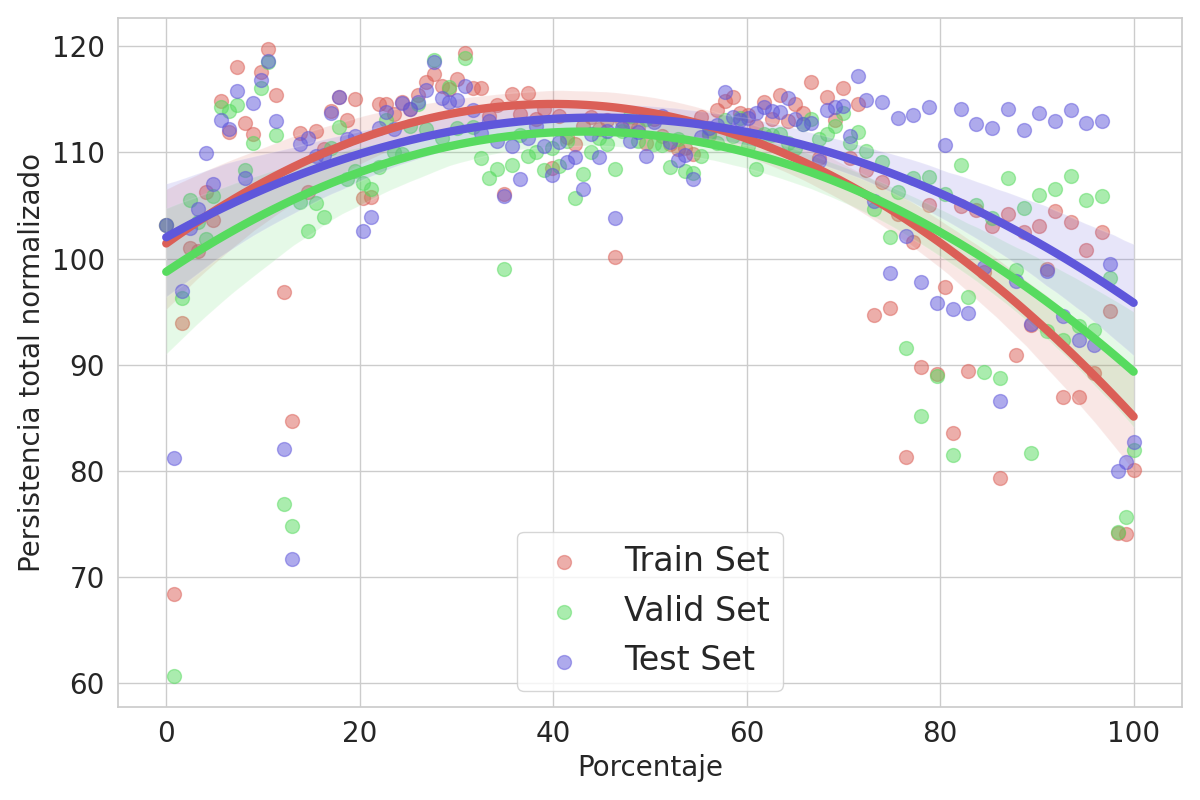
\includegraphics[width=\linewidth]{img/mm_set_base_norm.png}
		\caption{Persistencia total normalizada según el porcentaje de avance en la red para los conjuntos de entrenamiento, validación y test.}
		\label{fig:mm_set_base_norm}
	\end{subfigure}
	\begin{subfigure}{.45\textwidth}
		\centering
		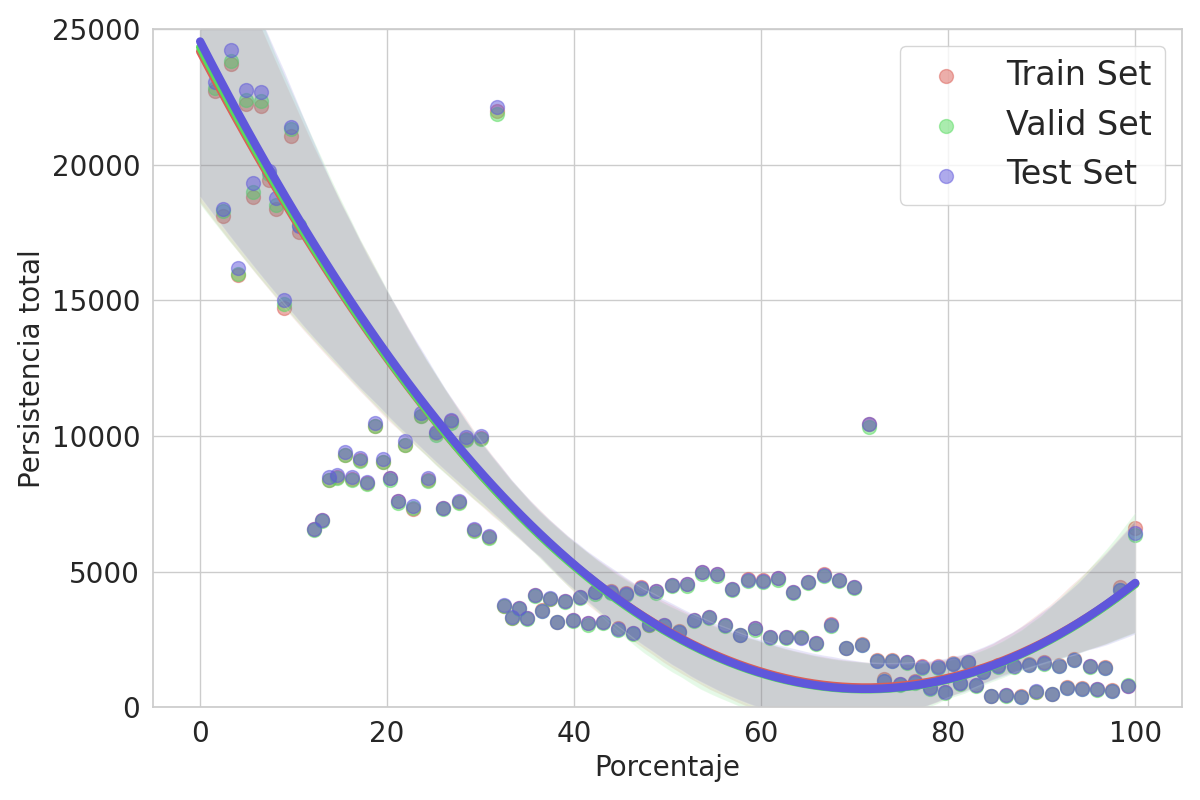
\includegraphics[width=\linewidth]{img/mm_set_trans.png}
		\caption{Persistencia total según el porcentaje de avance en la red con aumento de datos para los conjuntos de entrenamiento, validación y test.}
		\label{fig:mm_set_trans}
	\end{subfigure}%
	\begin{subfigure}{.45\textwidth}
		\centering
		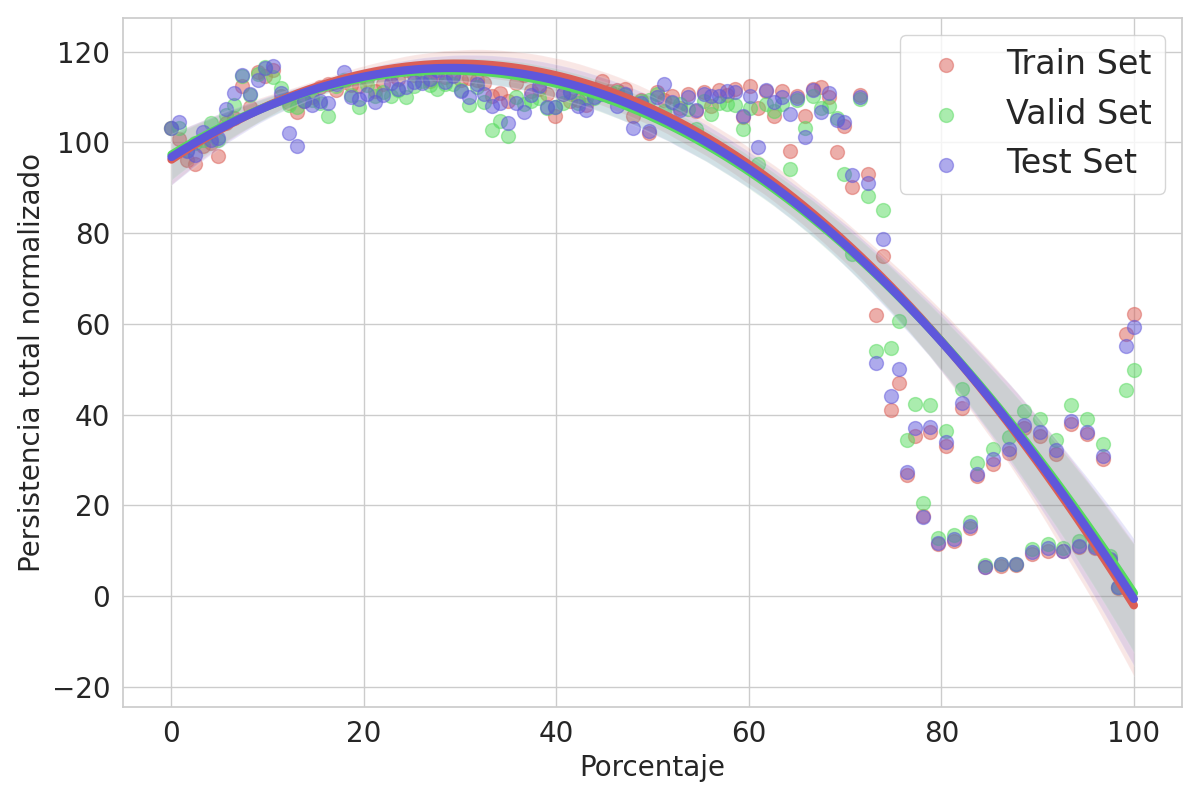
\includegraphics[width=\linewidth]{img/mm_set_trans_norm.png}
		\caption{Persistencia total normalizada según el porcentaje de avance en la red con aumento de datos para los conjuntos de entrenamiento, validación y test.}
		\label{fig:mm_set_trans_norm}
	\end{subfigure}
	\caption{Comparación de la persistencia total (a, c) y la persistencia total normalizada (b, d) para los conjuntos de entrenamiento, validación y test para la especificidad Marca-Modelo. Las Subfiguras (a) y (c) representan el modelo base, mientras que las Subfiguras (b) y (d) representan el modelo con aumento de datos.}
	\label{fig:mm-set}
\end{figure}

Las Figuras \ref{fig:m-set} y \ref{fig:mm-set} muestran cómo las redes mejor entrenadas obtienen una coincidencia mayor entre los distintos subconjuntos de datos empleados típicamente en el entrenamiento de las CNNs, lo que indica un mejor aprendizaje de la variedad subyacente de la que parten los datos.

\subsection{Propuesta de mejora: regularización topológica}
\label{subsec:proposal}

\subsubsection{Mejora en clasificación}

\begin{table}[H]
	\centering
	\begin{adjustbox}{width=0.8\textwidth}
		\begin{tabular}{|c|c|c|c|c|c|}
			\hline
			\textbf{Métrica} & $\alpha$ & \textbf{Exactitud} & \textbf{Precisión} & \textbf{Sensibilidad} & \textbf{F1-Score} \\
			\hline
			EfficientNet-B0 Base & - & 0.9505 & 0.9462 & 0.9386 & 0.9423 \\
			\hline
			EfficientNet-B0 Fine-Tune & 0.0 & 0.9598 & 0.9512 & 0.9445 & 0.9478 \\
			\hline
			EfficientNet-B0 Fine-Tune & 0.001 & 0.9598 & 0.9496 & 0.9448 & 0.9472 \\
			\hline
			EfficientNet-B0 Fine-Tune & 0.005 & \textbf{0.9659} & \textbf{0.9545} & \textbf{0.9514} & \textbf{0.9529} \\
			\hline
			EfficientNet-B0 Fine-Tune & 0.01 & 0.9598 & 0.9517 & 0.9481 & 0.9499 \\
			\hline
			EfficientNet-B0 Fine-Tune & 0.05 & 0.9536 & 0.9515 & 0.9412 & 0.9462 \\
			\hline
			EfficientNet-B0 Fine-Tune & 0.1 & 0.9567 & 0.9475 & 0.9413 & 0.9444 \\
			\hline
			EfficientNet-B0 Fine-Tune & 0.5 & 0.9505 & 0.9486 & 0.9369 & 0.9426 \\
			\hline
			EfficientNet-B0 Fine-Tune & 1.0 & 0.9505 & 0.9453 & 0.9413 & 0.9432 \\
			\hline
		\end{tabular}
	\end{adjustbox}
	\caption{Comparación de 4 Modelos sobre 4 Métricas}
	\label{tab:model_comparison_test}
\end{table}

\begin{table}[H]
	\centering
	\begin{adjustbox}{width=0.8\textwidth}
		\begin{tabular}{|c|c|c|c|c|c|}
			\hline
			\textbf{Métrica} & $\alpha$ & \textbf{Exactitud} & \textbf{Precisión} & \textbf{Sensibilidad} & \textbf{F1-Score} \\
			\hline
			DenseNet-121 Base & - & 0.9185 & 0.9077 & 0.9126 & 0.9101 \\
			\hline
			DenseNet-121 Fine-Tune & 0.0 & 0.9333 & 0.9220 & 0.9286 & 0.9253 \\
			\hline
			DenseNet-121 Fine-Tune & 0.001 & 0.9333 & 0.9220 & 0.9286 & 0.9253 \\
			\hline
			DenseNet-121 Fine-Tune & 0.005 & 0.9370 & 0.9269 & 0.9336 & 0.9302 \\
			\hline
			DenseNet-121 Fine-Tune & 0.01 & 0.9333 & 0.9220 & 0.9286 & 0.9253 \\
			\hline
			DenseNet-121 Fine-Tune & 0.05 & 0.9370 & 0.9284 & 0.9334 & 0.9308 \\
			\hline
			DenseNet-121 Fine-Tune & 0.1 & \textbf{0.9407} & \textbf{0.9384} & \textbf{0.9414} & \textbf{0.9399} \\
			\hline
			DenseNet-121 Fine-Tune & 0.5 & 0.9370 & 0.9297 & 0.9330 & 0.9313 \\
			\hline
			DenseNet-121 Fine-Tune & 1.0 & 0.9000 & 0.8997 & 0.8945 & 0.8970 \\
			\hline
		\end{tabular}
	\end{adjustbox}
	\caption{Comparación de 4 Modelos sobre 4 Métricas}
	\label{tab:model_comparison_test}
\end{table}

\subsubsection{Mejora en transferibilidad}




\section{Discusión}

\endinput
%--------------------------------------------------------------------
% FIN DEL CAPÍTULO. 
%--------------------------------------------------------------------
